% !TeX spellcheck = sk_SK-Slovak
% !TeX root = statnicaEKT.tex
%%%======= Balicky ======%%
%\documentclass[12pt,a4paper]{sablonaMVA}
%\usepackage{graphicx}
%\usepackage{multirow}
%\usepackage{multicol}
%\usepackage{array}
%\usepackage{lipsum}
%\usepackage{blindtext}
%\usepackage{nicematrix}
%\usepackage{wrapfig}
%\usepackage{caption}
%\usepackage{subcaption}
%\usepackage{amsmath}
%\usepackage{float}
%\usepackage{amssymb}
%\usepackage{hyperref}
%\usepackage{siunitx}
%\usepackage{relsize}
%\sisetup{detect-all}
%\usepackage[english,slovak]{babel}  \usepackage[T1]{fontenc}
%\usepackage{booktabs}
%\usepackage{makecell}
%\usepackage{numerica}
%\usepackage[normalem]{ulem}
%\usepackage{tikz}
%\usepackage{etoolbox}
%\usepackage{enumitem}
%\preto\tabular{\shorthandoff{-}}

%====== Vyplňte údaje ======
%\documentclass[a4paper,12pt]{article}
%\usepackage[a4paper,margin=2cm]{geometry}
%\usepackage[most]{tcolorbox}
%\usepackage{xcolor}
%\usepackage{ragged2e}
%
%\newcommand{\uloosdot}[1]{%
%	\tikz[baseline=(todotted.base)]{
%		\node[inner sep=1pt,outer sep=0pt] (todotted) {#1};
%		\draw[loosely dotted] (todotted.south west) -- (todotted.south east);
%	}%
%}%
%
%\begin{document}
%% ===================== HLAVIČKA DOKUMENTU =====================
%% Definícia farieb podľa predlohy
%\definecolor{nadpisblue}{RGB}{18,32,115}
%\definecolor{boxgray}{RGB}{230,230,230}
%\definecolor{boxborder}{RGB}{90,110,180}
%
%% Pravý horný roh
%\begin{flushright}
%	\small
%	\textbf{BPC-VFT, Vysokofrekvenční technika}\\
%	Vypracované otázky k SZZ od družiny vajčakov  
%\end{flushright}
%\raggedright

% ===============================================================
%\section*{\normalsize OTÁZKY}
%	\begin{itemize}
%		\item[1.] Základní typy mikrovlnných integrovaných obvodů (hybridní, monolitické MIO, MIO se soustředěnými parametry). Vlnovod integrovaný do substrátu, jeho provedení a základní vlastnosti.
%		Všechny potřebné údaje jsou uvedeny v příloze Důležité údaje a čísla.   
%		%\vspace*{-1.5mm}
%		\item[2.] Rezonátory (rezonátory z úseků vedení, dutinové rezonátory, planární a dielektrické rezonátory). Zásady buzení vlnovodů a dutinových rezonátorů sondou, proudovou smyčkou a štěrbinou.
%		%\vspace*{-1.5mm} 
%		\item[3.] Výkonové děliče, směrové vazební členy a jejich základní technické parametry.
%	\end{itemize}
\part{BPC-VFT - Vysokofrekvenční technika }
%\chapter{Okruhy:}

{\huge Otázky:}

\begin{enumerate}
	\item Otázka - Paralelní a sériové rezonanční obvody. Přizpůsobení paralelním rezonančním obvodem a L-článkem. Vázané rezonanční obvody. Filtry se soustředěnou selektivitou. Směrování a řízení úrovně vf signálu. 
	\item Otázka - Kritérium a kružnice stability. Šumové číslo. Šum atenuátoru a zesilovače. Dynamický rozsah DR a SFDR. Linearizovaný a velkosignálový zesilovač. Nízkošumový zesilovač, šumové přizpůsobení. 
	\item Otázka - Parametry směšovačů. Zpětnovazební oscilátor, podmínka oscilací. Tříbodová zapojení, přeladitelnost. Vlastnosti oscilátorů. Typy PLL syntezátoru, princip DDS, jejich spektrální vlastnosti.
	
\end{enumerate}

\newpage
	
% 	\section{\normalsize Paralelní a sériové rezonanční obvody. Přizpůsobení paralelním rezonančním obvodem a L-článkem. Vázané rezonanční obvody. Filtry se soustředěnou selektivitou. Směrování a řízení úrovně vf signálu.}
\chapter{Otázka VFT 1.}
	\textbf{Využitie rezonančných LC obvodov:}
	\begin{itemize}[label=$\rightarrow$]
		%\vspace{-2mm}
		\item selektívne vlastnosti - filtry
		\item transformácia impedancie - impedančné a výkonové prispôsobenia
		%\vspace*{-4mm}
	\end{itemize}
	
	\subsubsection{Sériový rezonančný obvod}
	%\vspace*{-2mm}
	\begin{itemize}[label=--]
		\item skladá zo sériového zapojenia ideálnych súčiastok R, L, C, pričom rezistor R vyjadruje straty reálneho kondenzátora a cievky.
		%%\vspace*{-2mm}
	\end{itemize}
	
	{\raggedright\textbf{Podmienky vzniku rezonancie:}}
	%\vspace*{-2mm}
	\begin{itemize}[label=--]
		\item rezonancia nastáva, keď $\mathbf{X_C = X_L}$
		\item reaktancia celkového obvodu $\mathbf{X = 0}$, navzájom sa vyrušia, obvod vykazuje iba odpor $R$
		\item pre výpočet rezonančného kmitočtu sa používa Thomsonov vzťah (\ref{eq:thomson}):
	\end{itemize}
	%\vspace{-1mm}
	\begin{equation}
		f_0 = \frac{1}{2\pi \sqrt{LC}}
		\label{eq:thomson}
	\end{equation}
	
	\subsubsection{Medzné kmitočty a priepustné pásmo}
		%\vspace*{-2mm}
	\begin{itemize}[label=--]
		\item po stranách sú definované dva medzné kmitočty $f_{c1}$ a $f_{c2}$, pre ktoré platí: $\mathbf{\abs{X} = R}$, je to frekvencia pri ktorej \textbf{prúd} poklesne o 3 dB
		\item pásmo medzi týmito medznými kmitočtami sa nazýva priepustné pásmo, $\mathbf{B = f_{c2}-f_{c1}}$
		%\vspace*{-4mm}
	\end{itemize}
	
	
	\begin{figure}[H]
	\centering
	\begin{subfigure}[t]{0.48\textwidth}
		\centering
		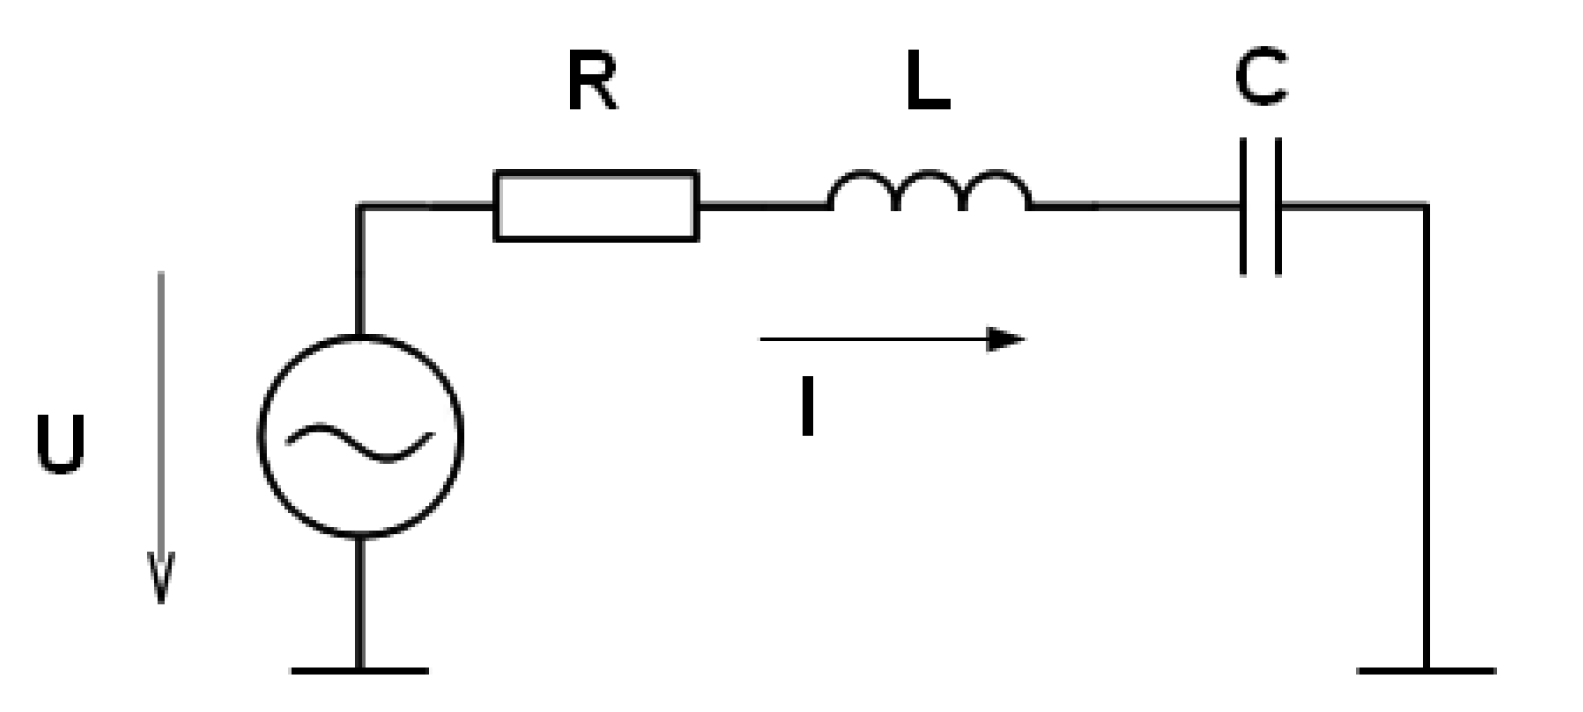
\includegraphics[scale=0.125]{Obrazky/VFT/seriovy_rezon_obvod.png}
		\caption{RLC obvod}
	\end{subfigure}
	\hfill
	\begin{subfigure}[t]{0.48\textwidth}
		\centering
		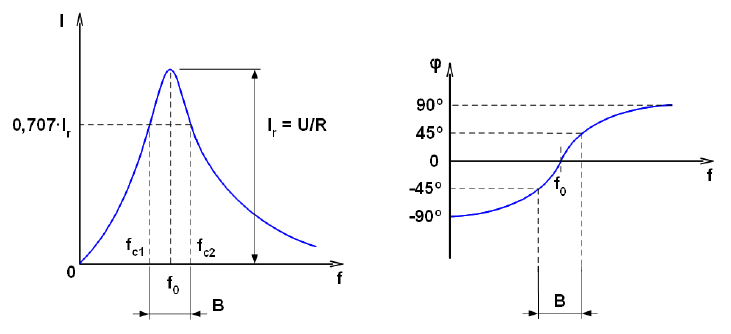
\includegraphics[scale=0.35]{Obrazky/VFT/rezonancna_krivka_a_faz_char_ser_RLC.png}
		\caption{Rezonančná krivka a fázová charakteristika}
	\end{subfigure}
	\caption{Sériový rezonančný obvod}
	\label{fig:seriovy_rlc}
	%\vspace{-4mm}
	\end{figure}
	
	{\raggedright \textbf{Selektivita}: schopnosť obvodu prepúšťať iba signály v určitom frekvenčnom pásme\\ }
	{\raggedright Pomer L/C:}
	\begin{itemize}[label = $\rightarrow$]
		%\vspace*{-2mm}
		\item vyššie L/C $\rightarrow$ menšia šírka pásma, väčšia strmosť frekvenčnej charakteristiky $\rightarrow$ lepšia selektivita
		\item nižšie L/C $\rightarrow$ väčšia šírka pásma $\rightarrow$ horšia selektivita
	\end{itemize}
	%\vspace*{-2mm}
	-- pri konšt. $R$ rastie $Q$ s $\sqrt{L/C}$
\begin{center}
	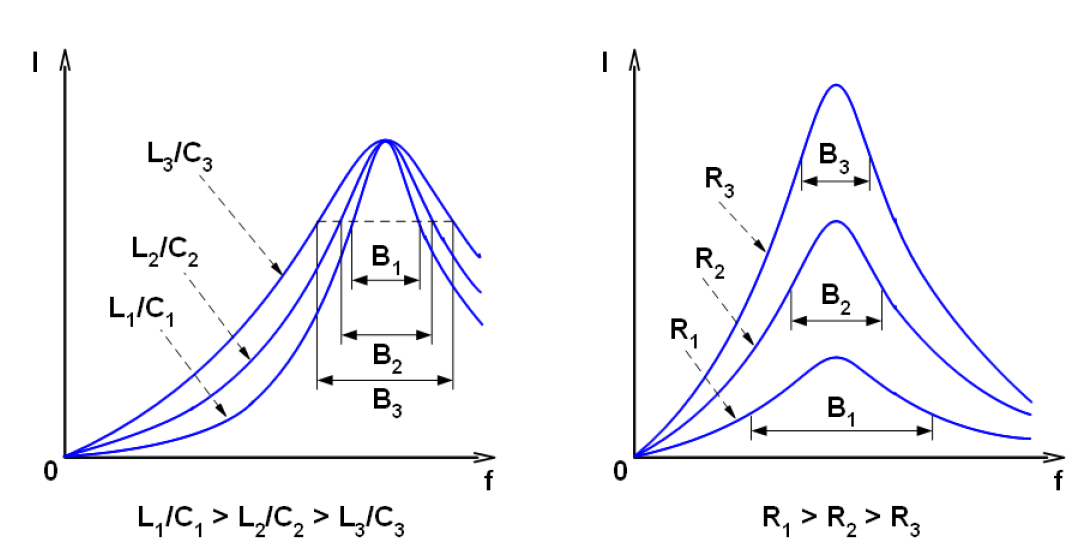
\includegraphics[scale=0.28]{Obrazky/VFT/selektivita_ser_RLC.png}\\
	{\small Obr. 1b: Šírka pásma (selektivita) sériového rezonančného obvodu}
\end{center}

		\noindent
	\begin{minipage}[t]{0.48\textwidth}
		\begin{equation}
			Q = \frac{X_L}{R} = \frac{X_C}{R}
		\end{equation}
	\end{minipage}
	\hfill
	\begin{minipage}[t]{0.48\textwidth}
		\begin{equation}
			B = \frac{f_0}{Q}
		\end{equation}
	\end{minipage}

	{\raggedright 	%\vspace*{4mm} Vplyv činiteľa jakosti Q:}
	\begin{itemize}[label = $\rightarrow$]
		%\vspace*{-2mm}
		\item vyššie Q $\rightarrow$ vyššia selektivita, užšia šírka pásma
		\item nižšie Q $\rightarrow$ horšia selektivita, väčšia šírka pásma
		%\vspace*{-2mm}
	\end{itemize}
	
		\subsubsection{Paralelný rezonančný obvod}
	%\vspace*{-2mm}
	\begin{itemize}[label=--]
		\item skladá zo paralelného zapojenia ideálnych súčiastok R, L, C, pričom rezistor R (vodivosť G) vyjadruje straty reálneho kondenzátora a cievky.
	\end{itemize}
	%\vspace{-1mm}
		{\raggedright\textbf{Podmienky vzniku rezonancie:}}
	%\vspace*{-2mm}
	\begin{itemize}[label=--]
		\item rezonancia nastáva, keď $\mathbf{X_C = X_L}$
		\item susceptancia celkového obvodu $\mathbf{X = 0}$, navzájom sa vyrušia, obvod vykazuje iba reálnu vodivosť $G$
		\item pre výpočet rezonančného kmitočtu sa používa Thomsonov vzťah (\ref{eq:thomson}):
	\end{itemize}
	%\vspace{-6.5mm}%-1mm
%	\begin{equation}
%		f_0 = \frac{1}{2\pi \sqrt{LC}}
%		\label{eq:thomson2}
%	\end{equation}
	
	\subsubsection{Medzné kmitočty a priepustné pásmo}
	%\vspace*{-3mm}%-2mm
	\begin{itemize}[label=--]
		\item po stranách sú definované dva medzné kmitočty $f_{c1}$ a $f_{c2}$ $\rightarrow$ frekvencia pri ktorej \textbf{napätie} poklesne o 3 dB
		\item pásmo medzi týmito medznými kmitočtami sa nazýva priepustné pásmo, $\mathbf{B = f_{c2}-f_{c1}}$
		%\vspace*{-4mm}
	\end{itemize}
	
	\begin{figure}[H]			
	\centering
		\begin{subfigure}[t]{0.48\textwidth}
			\centering
			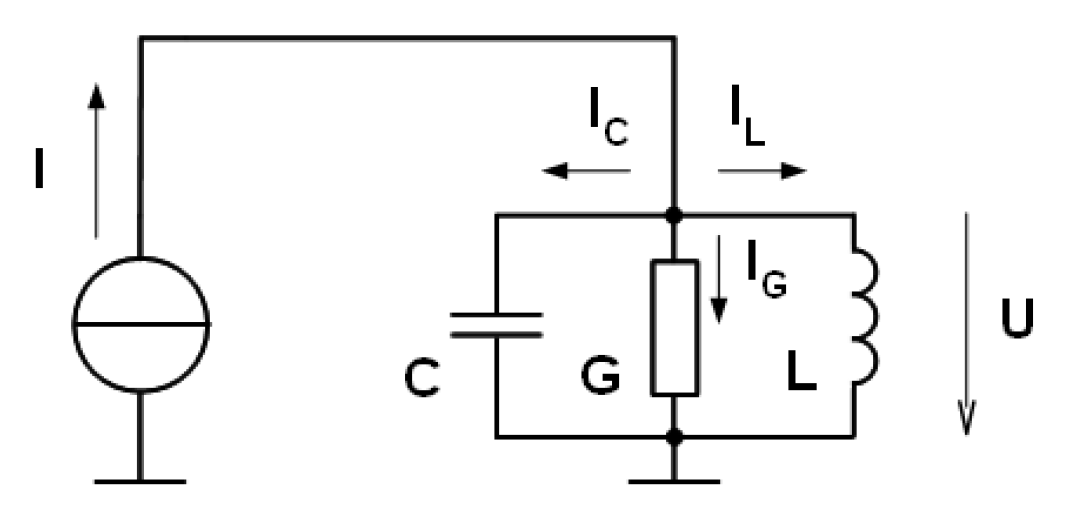
\includegraphics[scale=0.175]{Obrazky/VFT/paralelny_rezon_obvod.png}
			\caption{RLC obvod}
		\end{subfigure}
		\hspace{-10mm}
		\begin{subfigure}[t]{0.48\textwidth}
			\centering
			\captionsetup{justification=centering}
			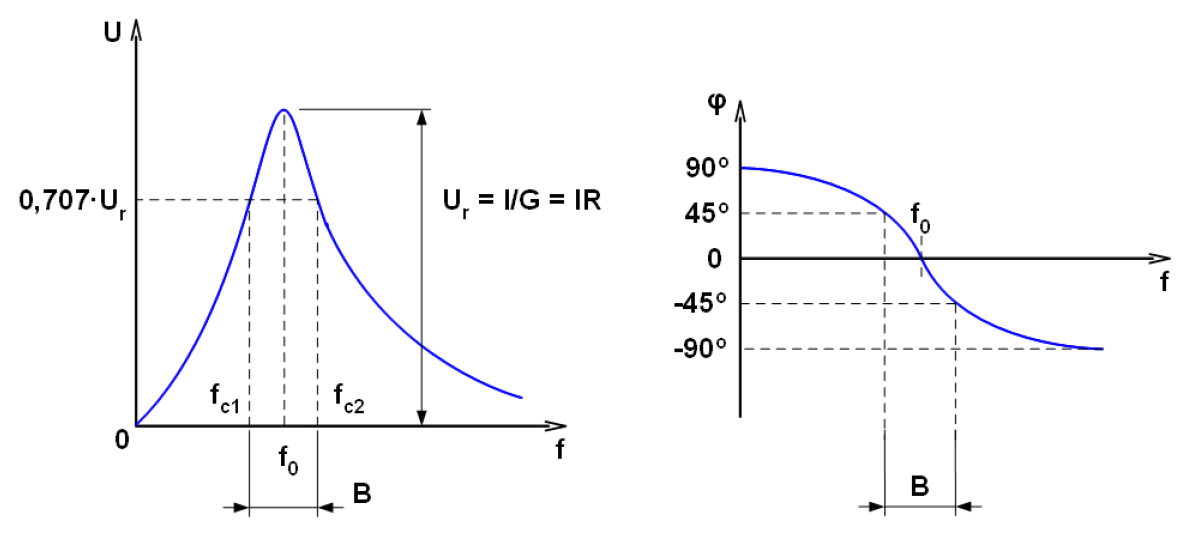
\includegraphics[scale=0.215]{Obrazky/VFT/rezonancna_krivka_a_faz_char_par_RLC.png}
			\caption{rezonančná krivka a fázová char.}
		\end{subfigure}
		\caption{Paralelný rezonančný obvod}
		\label{fig:paralel_rlc}
	\end{figure}
	
	{\raggedright Pomer L/C:}
	\begin{itemize}[label = $\rightarrow$]
		%\vspace*{-2mm}
		\item vyššie L/C $\rightarrow$ väčšia šírka pásma, $\rightarrow$ horšia selektivita
		\item nižšie L/C $\rightarrow$ menšia šírka pásma, väčšia strmosť $\rightarrow$ lepšia selektivita
	\end{itemize}
	%\vspace*{-2mm}
	-- pri konšt. $R$ rastie $Q$ s poklesom $\sqrt{L/C}$ 
	\begin{center}
		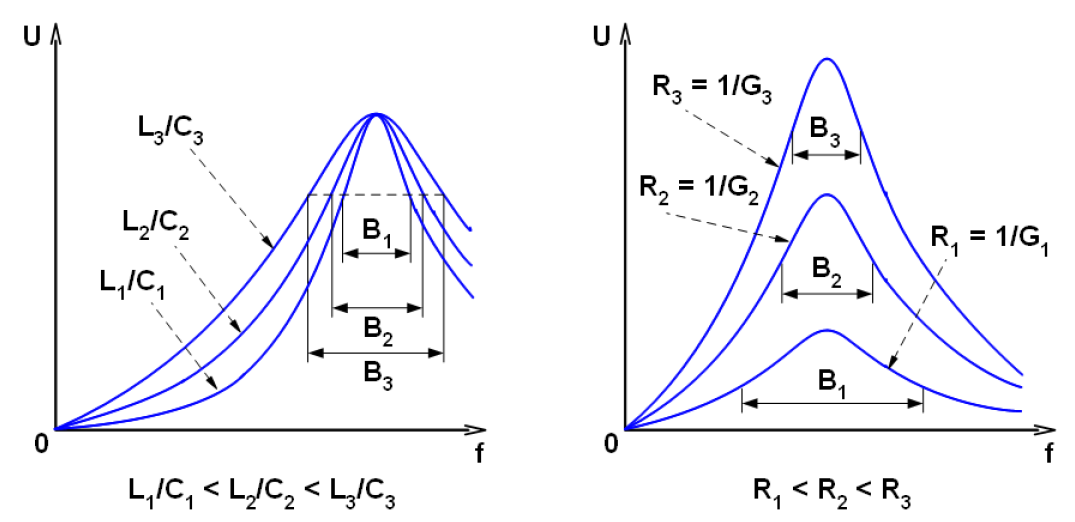
\includegraphics[scale=0.275,]{Obrazky/VFT/selektivita_par_RLC.png}\\
		{\small Obr. 2b: Šírka pásma (selektivita) paralelného rezon. obvodu}
	\end{center}
	
\noindent
\begin{minipage}[t]{0.3\textwidth}
	\begin{equation}
		Q = \frac{R}{X_L} = \frac{R}{X_C}
	\end{equation}
\end{minipage}
\hfill
\begin{minipage}[t]{0.3\textwidth}
	\begin{equation}
		Q = \frac{R}{\sqrt{L/C}}
	\end{equation}
\end{minipage}
\hfill
\begin{minipage}[t]{0.3\textwidth}
	\begin{equation}
		B = \frac{f_0}{Q}
	\end{equation}
\end{minipage}

	{\raggedright 	%\vspace*{4mm} Vplyv činiteľa jakosti Q:}
	\begin{itemize}[label = $\rightarrow$]
		%\vspace*{-2mm}
		\item vyššie Q $\rightarrow$ vyššia selektivita, väčšia strmosť, užšie pásma
		\item nižšie Q $\rightarrow$ horšia selektivita, širšie pásmo
	\end{itemize}
	%\vspace*{-2.5mm}
	\hspace{5mm}-- Q rastie s R

	\subsubsection{Impedančné a výkonové prispôsobenie}
	
	\subsubsection{Činiteľ odrazu}
	\begin{figure}[H]
		\centering
		\begin{minipage}[c,t]{0.325\textwidth}
			\centering
			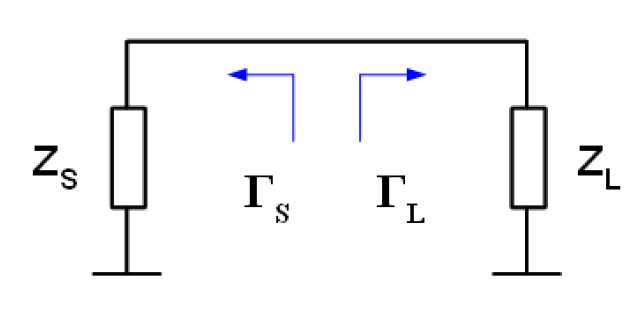
\includegraphics[width=\linewidth]{Obrazky/VFT/cinitel_odrazu.png}
			\caption{Činiteľ odrazu}
		\end{minipage}
		\hspace{-20mm}
		\begin{minipage}[c,t]{0.5\textwidth}
			\begin{equation}
				\Gamma_L = \frac{Z_L-Z_S}{Z_L+Z_S}
			\end{equation}
			%\vspace*{0mm}
			\begin{equation}
				\Gamma_S = \frac{Z_S-Z_L}{Z_S+Z_L}
			\end{equation}
		\end{minipage}
	\end{figure}
	{\raggedright
	$Z_S$ -- impedancia zdroja (source) $Z_L$ -- impedancia záťaže (load), $\Gamma$ -- činiteľ odrazu
	\begin{itemize}[label = ]
		%\vspace*{-2mm}
		\item  $\mathbf{\Gamma}$ je definovaný ako pomer odrazenej a dopadajúcej vlny na rozhraní impedancii $Z_s$ a $Z_L$
		\item \hspace{-1mm}$\mathbf{\abs{\Gamma}}$ = 0 -- dokonalé prispôsobenie, žiadny odraz
	\end{itemize}}
	
	\subsubsection{Podmienka impedančného prispôsobenia}
	\begin{itemize}[label=--]
	%\vspace{-2.5mm}
	\item reálne i komplexné zložky impedancie generátora aj záťaže musia byť rovnaké
	\item výsledný činiteľ odrazu je potom nulový, nedochádza k žiadnym odrazom
	\end{itemize}
	%\vspace{-2mm}
	\begin{equation}
		Z_S = Z_L
		\label{eq:impedan_prisp}
		%\vspace{-3mm}
	\end{equation} 
	
	\subsubsection{Podmienka výkonového prispôsobenia}
	\begin{itemize}[label=--]
		%\vspace{-2.5mm}
		\item vzájomná komplexná združenosť oboch impedancií
	\end{itemize}
	%\vspace{-2mm}
	\begin{equation}
		Z_S = Z_L^*
		\label{eq:výkon_prisp}
		%\vspace{-2mm}
	\end{equation}
	\begin{itemize}[label=--]
		\item výsledný činiteľ odrazu:
	\end{itemize}
	%\vspace{-2.5mm}
	\begin{equation}
		\Gamma = \frac{Z_L-Z_L^*}{Z_L+Z_L^*}
	\end{equation}
	%\vspace*{1mm}
	V prípade, že budú obe reaktancie nulové ($Z_S$ a $Z_L$ ma iba reálnu zložku), činiteľ odrazu bude nulový $\rightarrow$ \textbf{výkonové prispôsobenie je zároveň impedančné prispôsobenie}.
	%\vspace*{-4mm}
	\subsubsection{Prispôsobenie paralelným rezonančným obvodom a L-článkom}
	\begin{itemize}[label=--]
		%\vspace*{-2.5mm}
		\item prispôsobenie impedancie funguje iba na rezonančnom kmitočte obvodu (poprípade v jeho blízkom okolí)
	\end{itemize}

	\begin{figure}[H]
		%\vspace{-2mm}
		\makebox[\textwidth]{%
			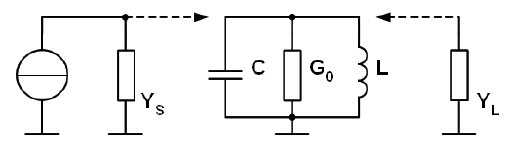
\includegraphics[scale=0.6]{Obrazky/VFT/paralel_rezon_obvod_transf.png}}
		\caption{Zapojenie paralelného rezonančného obvodu pre prispôsobenie obvodu}
	\end{figure}
	
	%\vspace{-5mm}
	\subsubsection{Vplyv pripojenia záťaže k paralelnému rezonančnému obvodu na rezonančný kmitočet a činiteľ jakosti}	
	\begin{itemize}[label=--]
		%\vspace{-2mm}
		\item pripojením záťaže k paralelnému rezonančnému obvodu dôjde k poklesu činiteľa jakosti~$Q$
		\begin{itemize}[label=$\rightarrow$]
			%\vspace*{-4mm}
			\item zväčší sa paralelná vodivosť
			\item zväčší sa šírka pásma $B$
			\item mierny posun rezonančného kmitočtu	
		\end{itemize}
		%\vspace*{-2mm}
		\item preto sa k rezonančnému obvodu pripojujú záťaže, ktoré majú čiste reálnu admitanciu
	\end{itemize}

	\subsubsection{Minimalizácia strát prenosu výkonu}	
	%\vspace{-2.5mm}
	\begin{itemize}[label=--]
		\item straty prenosom výkonu sú minimálne pri:
		\begin{itemize}[label=$\rightarrow$]
			%\vspace*{-4mm}
			\item veľkej hodnote činiteľa jakosti nezaťaženého obvodu $Q_0$ a súčasne nízkej hodnote činiteľa jakosti zaťaženého obvodu $Q$
			\item výkonovom prispôsobení zdroja a záťaže ($G_S$ = $G_L$)
		\end{itemize}
	\end{itemize}
	\begin{equation}
		\eta = \left(1-\frac{Q}{Q_0}\right)^2
	\end{equation}
	
	\subsubsection{Podmienka vysokej účinnosti}	
	\begin{equation}
		Q_0 \gg Q_L
	\end{equation}
	
	\begin{itemize}[label=--]
		\item nezaťažený obvod musí mať vysoký činiteľ jakosti $Q_0$
		\item zaťažený obvod musí mať nízky činiteľ jakosti $Q_L$
	\end{itemize}
	%\vspace{-2.5mm}
	\subsubsection{Obmedzenie vplyvu záťaže}
	%\vspace{-2mm}
	\begin{itemize}[label=--]
		\item záťaž sa nepripája napriamo, ale pomocou troch spôsobov:
			\begin{itemize}[label=$\rightarrow$]
				%\vspace*{-4mm}
				\item \textbf{na odbočku cievky}
				\item \textbf{kapacitným deličom}
				\item \textbf{väzobním vinutím}
			%	\item pre každý zo spôsobou sa definuje transformačný činiteľ $p$ (platí $p$ < 1)
			\end{itemize}
			%\vspace{-2mm}
		\item modul admitancie záťaže je mnohonásobne väčší než modul admitancie rezonančného obvodu v bodoch pripojenia záťaže
		\item pridávanie záťaže, ktoré majú čiste reálnu admitanciu
		\item ak sa pripája imaginárna zložka $\rightarrow$ započítať to do rezonančného obvodu, aby rezonancia bola na požadovanom kmitočte
	\end{itemize}
	
	\subsubsection{Spôsoby naviazania záťaže}
	
		\begin{itemize}[label=--]
		%\vspace*{-2mm}
		\item pre každý zo spôsobou sa definuje transformačný činiteľ $p$ (platí $p$ < 1)
		\item pripojením záťaže paralelne k rezonančnému obvodu cez viazanie -- jej hodnota sa násobí kvadrátom transformačného činiteľa na hodnotu $p^2 Y_L$
	\end{itemize}
	
	
	\begin{figure}[H]
		%\vspace{-2mm}
		\makebox[\textwidth]{%
			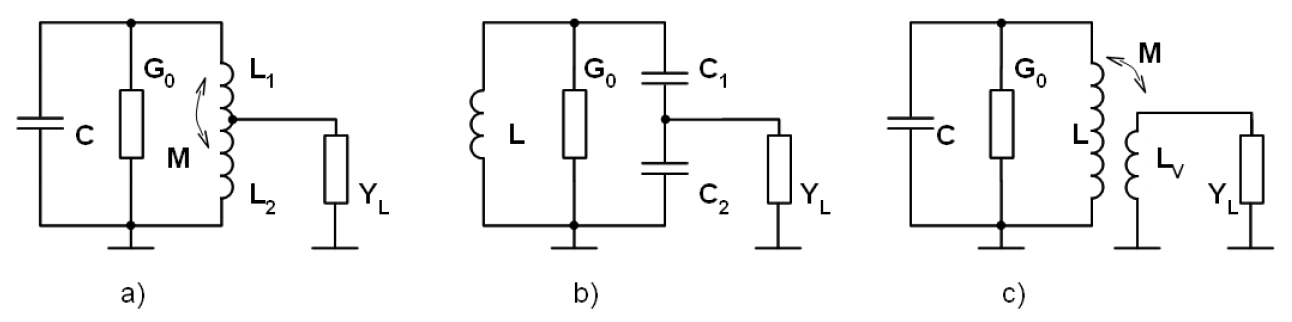
\includegraphics[scale=0.45]{Obrazky/VFT/sposoby_pripojenia_zataze_k_paralel_rezon_obvosu.png}}
		\caption{Zapojenie paralelného rezonančného obvodu pre prispôsobenie obvodu}
	\end{figure}
	
	\noindent
	\begin{minipage}[t]{0.32\textwidth}
		\raggedright
		\textbf{a) Na odbočku cievky}
		
		%\vspace*{-2mm}
		\begin{equation}
			p = \frac{L_2 + M}{L_1 + L_2} \cong \frac{U_L}{U_0}
		\end{equation}
	\end{minipage}
	\hfill
	\begin{minipage}[t]{0.32\textwidth}
		\raggedright
		\textbf{b) Kapacitným deličom}
		
		%\vspace*{-2mm}
		\begin{equation}
			p = \frac{C_1}{C_1 + C_2} \cong \frac{U_L}{U_0}
		\end{equation}
	\end{minipage}
	\hfill
	\begin{minipage}[t]{0.32\textwidth}
		\raggedright
		\textbf{c) Väzobným vinutím}
		
		%\vspace*{-2mm}
		\begin{equation}
			p = \frac{L_V + M}{L} \cong \frac{U_L}{U_0}
		\end{equation}
	\end{minipage}
	
	\subsubsection{Paralelný rezonančný obvod ako prispôsobovací článok}

	\begin{figure}[H]
		\centering
		\begin{minipage}[c,t]{0.4\textwidth}
			\centering
			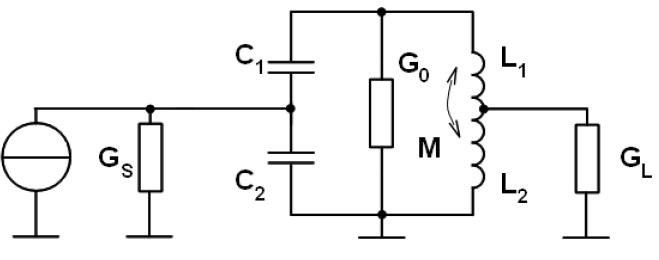
\includegraphics[width=\linewidth]{Obrazky/VFT/prisp_gen_k_zatazI_paralel_rezon.png}
			\caption{Prispôsobenie generátora k \\záťaži pomocou paralel. rezonančného obvodu}
		\end{minipage}
		\hspace{-20mm}
		\begin{minipage}[c,t]{0.5\textwidth}
			\begin{equation}
				G_S = \frac{1}{R_S}
			\end{equation}
			%\vspace*{0mm}
			\begin{equation}
				G_L = \frac{1}{R_L}
			\end{equation}
		\end{minipage}
	\end{figure}
	
	
	\begin{itemize}[label=--]
	\item podmienka výkonového prispôsobenia: $Y_S = Y_L^*$
	%\vspace{-4mm}
	\end{itemize}
	\begin{itemize}[label=--]
	\item pri čisto reálnych admitanciách platí: $G_S = G_L$
	\end{itemize}
		

\textbf{Transformácia vodivosti}
	\begin{itemize}[label=--]
		%\vspace{-2mm}
		\item vodivosť generátora sa transformuje:
			\begin{itemize}[label=$\rightarrow$]
				%\vspace{-4mm}
				\item kapacitným deličom s pomerom $p_1$
			\end{itemize}
			%\vspace{-2mm}
		\item vodivosť záťaže sa transformuje: 
			\begin{itemize}[label=$\rightarrow$]
				%\vspace{-4mm}
				\item odbočkou na cievke s pomerom $p_2$
				%\vspace{-2mm}
			\end{itemize}
	\end{itemize}
			
	\begin{figure}[H]
		%\vspace{-2mm}
		\makebox[\textwidth]{%
			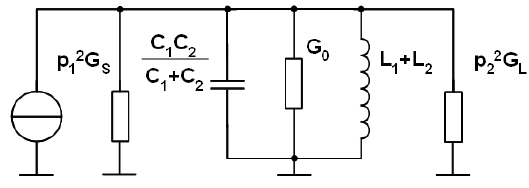
\includegraphics[scale=0.45]{Obrazky/VFT/prisp_gen_k_zatazI_paralel_rezon_nahrada.png}}
		\caption{Prispôsobenie generátora k záťaži - náhradná schéma zapojenia}
	\end{figure}
		
		
	{\raggedright-- po transformácií platí podmienka:}\\
	%\vspace{-5mm}
	\begin{equation}
		p_1^2 G_S = p_2^2 G_L
	\end{equation}
	-- vhodnou voľbou transformačných pomerov $p_1$ a $p_2$\\
%	%\vspace{2mm}
%{\raggedright \textbf{Vlastnosti prispôsobenia}}\\
%	%\vspace{-2.5mm}
%	\begin{itemize}[label=--]
%		\item prispôsobenie funguje iba v úzkom okolí rezonančného kmitočtu $f_0$
%		\item ide o úzkopásmový prispôsobovací obvod
%		\item rezonančný obvod má selektívne vlastnosti 
%	\end{itemize}
	%\vspace{2mm}
{\raggedright \textbf{Vplyv strát rezonančného obvodu}}\\	
	%\vspace{-4mm}
	\begin{itemize}[label=--]
	\item výkonové prispôsobenie nie je ideálne kvôli vlastnej vodivosti obvodu $G_0$ (súvisí s činiteľom jakosti $Q_0$)
	\item výsledná vodivosť zaťaženého obvodu
	\end{itemize}
	
	\begin{equation}
		G = p_1^2 G_s + G_0 + p_2^2G_L
	\end{equation}
	
	\begin{itemize}[label=--]
		\item zo vzťahu možno určiť:
			\begin{itemize}[label=$\rightarrow$]
			%\vspace{-3mm}
			\item činiteľ jakosti zaťaženého obvodu $Q$
			\item účinnosť
			\item vložený útlm
		\end{itemize}
	\end{itemize}	
	
	{\raggedright \textbf{Ideálne bezstratové prispôsobenie}}\\
	%\vspace{-3mm}
	\begin{itemize}[label=--]
		\item dokonalé bezstratové prispôsobenie by bolo možné iba pri $G_0 = 0$
		\item podmienka by platila pri ideálnych bezstratových súčiastkach $L$ a $C$
	\end{itemize}	
		
	\newpage
	\subsubsection{Transformácia L článkom}
	Vlastnosti reaktančných prispôsobovacích obvodov:
	%\vspace*{-2mm}
	\begin{itemize}[label=--]
		\item úzkopásmove
		\item požadovaný efekt je dosiahnutý ideálne na jednom kmitočte alebo v jeho bližšom okolí 
		\item nízke straty (pri použití súčiastok s vysokou jakosťou $Q$)
	\end{itemize}
	
	\begin{figure}[H]
	%\vspace{-2mm}
	\makebox[\textwidth]{%
		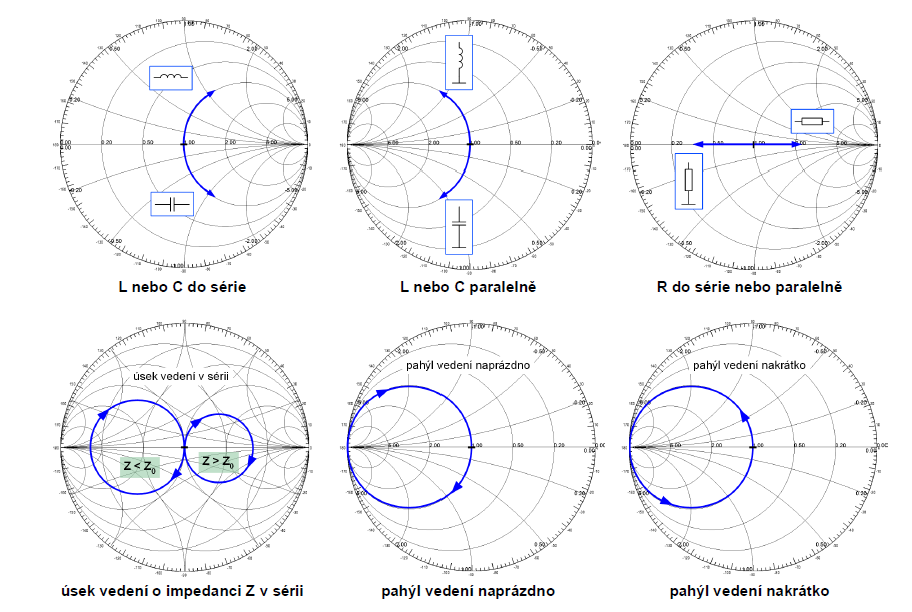
\includegraphics[scale=0.6]{Obrazky/VFT/pohyb_cinitela_odrazu.png}}
	\caption{Pohyb činiteľa odrazu obvodových prvkov}
	\end{figure}
	
	\subsubsection{Prispôsobenie záťaže pomocou L článku}
	\begin{itemize}[label=--]
		\item najjednoduchší prispôsobovací obvod, zložený z jedného kondenzátora a jednej cievky, ktorý môže byť zapojený v štyroch rôznych konfiguráciách
	\end{itemize}
	
	\begin{figure}[H]
	%\vspace{-2mm}
		\makebox[\textwidth]{%
			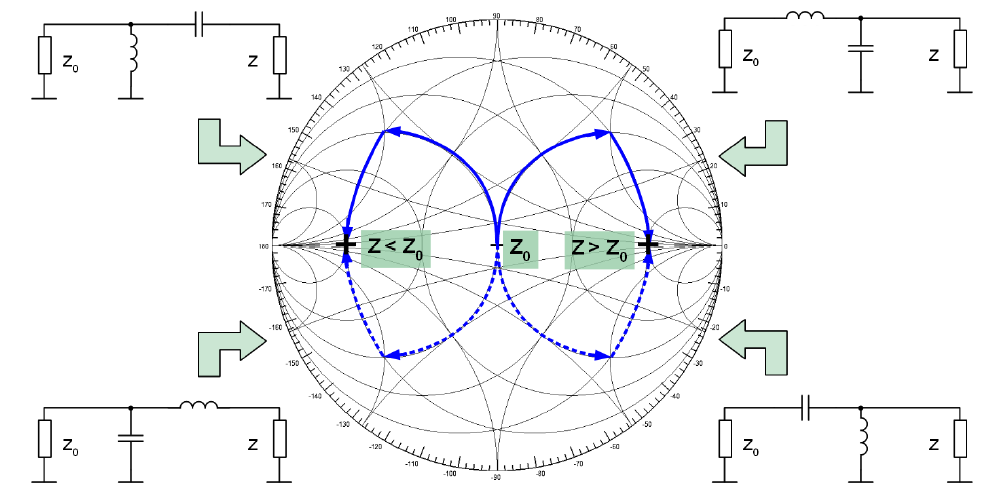
\includegraphics[scale=0.6]{Obrazky/VFT/prisposobenie_zataze_pomocou_l_clanku.png}}
		\caption{Pohyb činiteľa odrazu obvodových prvkov}
	\end{figure}
	
	\subsubsection{Viazané rezonančné obvody}
	%\vspace*{-2mm}
%	- pri použití jednoduchého rezonančného obvodu sme obmedzený malou selektivitou, ktorá závisí na činiteli jakosti
%	- použitím viacero rezonančných obvodov s vhodnými väzbami dostaneme selektívny obvod (pásmovú priepusť) s väčšou šírkou pásma a strmejším zlomom prenosovej charakteristiky na medzných kmitočtoch. 
%	
%	Možné väzby:
%				- väzba elektrickým poľom (väzobnými kondenzátorom) - 
%				- väzba magnetickým poľom
%					1.) väzobnou cievkou
%					2.) vzájomnou indukčnosťou dvoch cievok
%				- väzba kombináciou el. a mag. poľa
%				
%	- veľkosť väzby je kvantifikovaná činiteľom väzby $m$
%	- pri nízkych hodnotách $m$ $\rightarrow$ voľná väzba
%	- $m$ blízke 1 $\rightarrow$ tesná väzba
%	
%	
%	\begin{figure}[H]
%	%\vspace{-2mm}
%	\makebox[\textwidth]{%
%		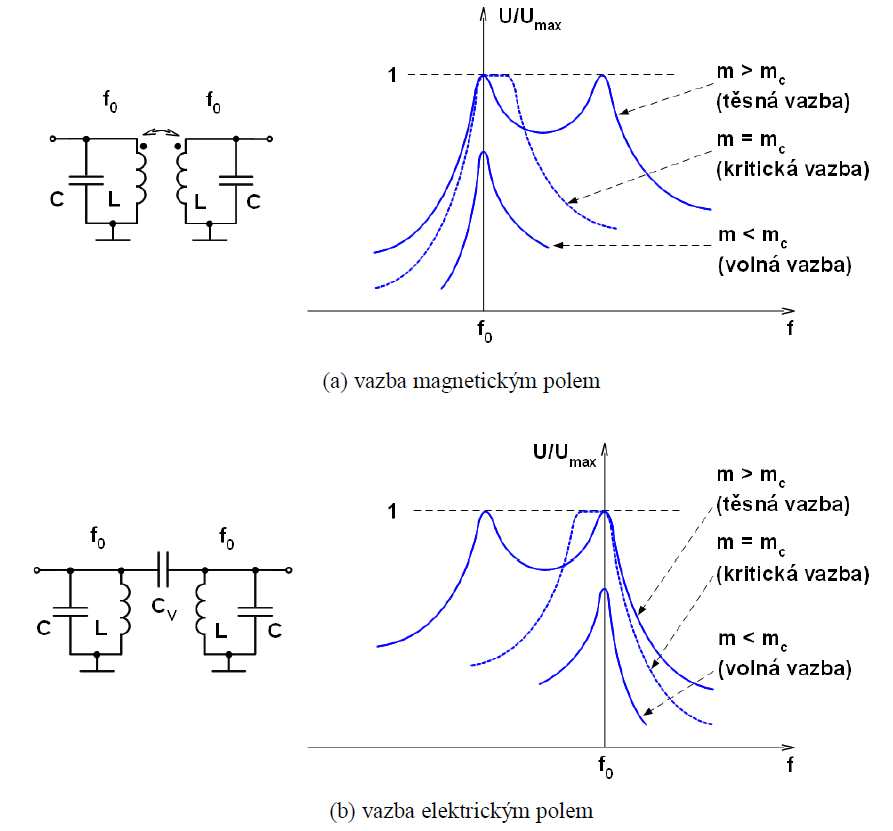
\includegraphics[scale=0.6]{Obrazky/VFT/rezonan_krivky_viazanych_obvodov.png}}
%	\captionsetup{justification=centering}
%	\caption{Rezonančné krivky viazaných rezonančných obvodov pre rôzne hodnoty činiteľa väzby $m$}
%	\end{figure}
%	
%	
%	
%	- pri väzbe menšej než je väzba kritická m < mc a pri m = mc má rezonančná kivka jeden vrchol
%	- pri väzbe m > mc má razonančná krivka dva vrcholy ktoré sa pri zväčšovaní činiteľa väzby od seba vzdiaľujú, i keď primárne a sekundárne obvody sú naladené stále na rovnáký rezonančný kmitočet $f_0$
%
%	pri väzbe magnetickým poľom - dochádza pri zvyšovaní m ku vzniku druhého vrcholu rezonančnej krivky na frekvencii vyššej než je $f_0$	
%	
%	Kritická väzba $m = m_c$
%	- stav kedy je väzba medzi dvoma rezonátormi práve tak silná, aby došlo k maximálnemu prenosu energie
%	- obvod ma najširšie možné pásmo pri zachovaní jedného vrcholu
%	- podobné krivkám jednouchého rezonančného obvodu (jeden vrchol)
%	
%	- zvyšovanie činiteľa väzby na rezonančnej krivky viazaných rezonančných obvodov
%	- rezonančné krivky budú mať dva vrcholy, ktoré sa pri zväčšovaní činiteľa väzby od seba vzdiaľujú
%	\newpage
	\begin{itemize}[label=--]
		\item jednoduchý rezonančný obvod má obmedzenú selektivitu závislú od činiteľa jakosti $Q$
		\item použitím viacerých viazaných rezonančných obvodov vzniká selektívny obvod (pásmová priepusť) s väčšou šírkou pásma a strmšou prenosovou charakteristikou na medzných kmitočtoch		
		\item možné typy väzieb:
		\begin{itemize}[label=$\rightarrow$]
			%\vspace{-3.5mm}
			\item väzba elektrickým poľom (väzobný kondenzátor)
			\item väzba magnetickým poľom:
			\begin{itemize}[label=$\triangleright$]
				 %\vspace{-2mm}
			\item väzobná cievka
				%\vspace{1mm}
				\item vzájomná indukčnosť dvoch cievok
			\end{itemize}
			\item kombinovaná väzba elektrickým a magnetickým poľom
		\end{itemize}
		%\vspace{-1mm}
		\item veľkosť väzby je určená činiteľom väzby $m_0$
		\item podľa veľkosti $m$:
		%\vspace{-3.5mm}
		\begin{itemize}[label=$\rightarrow$]
			\item malé $m$ $\rightarrow$ voľná väzba
			\item $m \approx 1$ $\rightarrow$ tesná väzba
		\end{itemize}
		
	\end{itemize}
	
	\begin{figure}[H]
		%\vspace{-2mm}
		\makebox[\textwidth]{%
			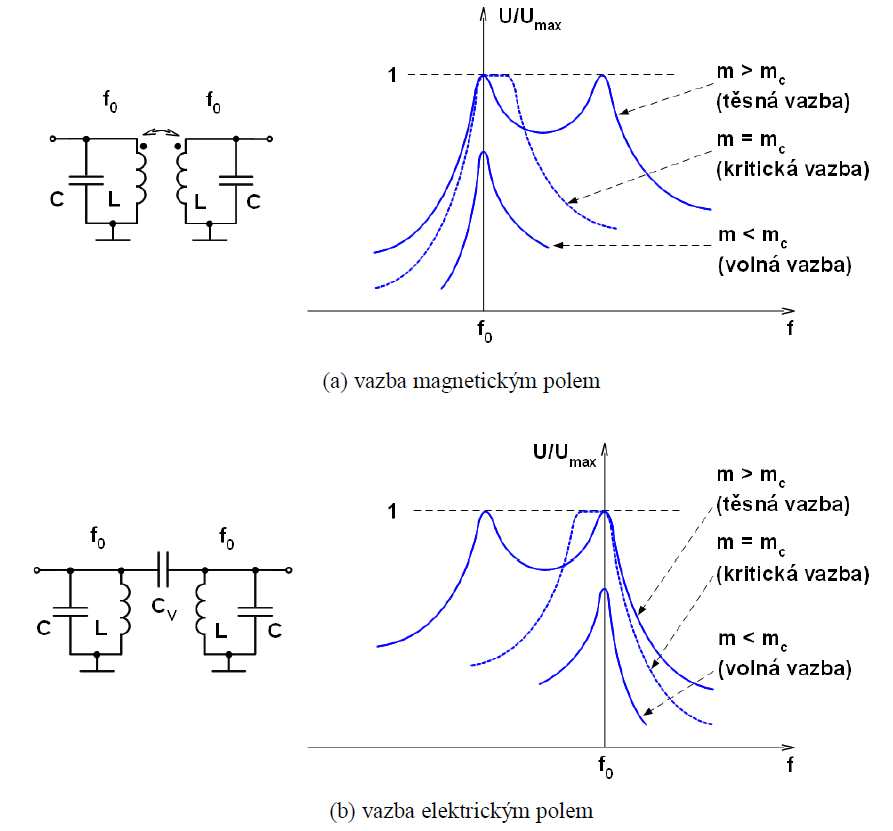
\includegraphics[scale=0.45]{Obrazky/VFT/rezonan_krivky_viazanych_obvodov.png}}
		\captionsetup{justification=centering}
		\caption{Rezonančné krivky viazaných rezonančných obvodov pre rôzne hodnoty činiteľa väzby $m$}
	\end{figure}
	
	\begin{itemize}[label=--]
		
		\item pri $m < m_c$ alebo $m = m_c$ má rezonančná krivka jeden vrchol
		
		\item pri $m > m_c$ vznikajú dva vrcholy rezonančnej krivky, ktoré sa so zvyšovaním $m$ od seba vzďaľujú
		
		\item pri magnetickej väzbe vzniká druhý vrchol rezonančnej krivky na frekvencii vyššej než $f_0$
	\end{itemize}
	
		\textbf{Kritická väzba}: $m = m_c$
	\begin{itemize}[label=--]
		%\vspace{-2.5mm}
		\item maximálny prenos energie medzi rezonátormi
		\item najširšie pásmo pri zachovaní jedného vrcholu
		\item charakteristika podobná jednoduchému rezonančnému obvodu
	\end{itemize}
	\subsubsection{Filtry se soustředěnou selektivitou}
	
	%\vspace*{-2mm}
	\begin{itemize}[label=--]
	\item pracujú na elektromechanických princípoch
	\item majú výhodnejšie vlastnosti v porovnaní s LC filtrami
	\item Výhody:
	\begin{itemize}[label=$\rightarrow$]
	%\vspace*{-4mm}
	\item menšie rozmery a hmotnosť,
	\item lepšie a reprodukovateľnejšie elektrické parametre 
	\item väčšia mechanická odolnosť, lepšie časová a tepelná stabilita
	\item nižšia cena, nie je potrebné nastavovať/dolaďovať
	\end{itemize}
	\end{itemize}
	\raggedright
	Dôležitým parametrom je činiteľ tvaru $k$
	\begin{equation}
		k = \frac{B_{60}}{B_6}
	\end{equation}
	kde $B_6$ je šírka pásma pre pokles prenosu filtra o 6 dB a $B_{60}$ pre pokles o 60 dB
		
	\begin{figure}[H]
	%\vspace{-2mm}
	\makebox[\textwidth]{%
		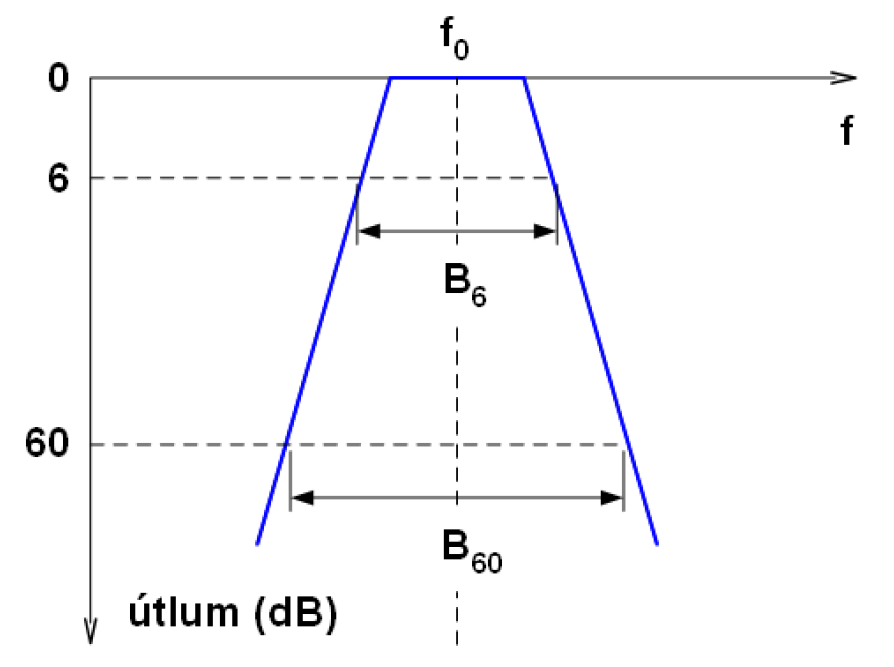
\includegraphics[scale=0.3]{Obrazky/VFT/cinitel_tvaru_filtru.png}}
	\captionsetup{justification=centering}
	\caption{Činiteľ tvaru filtra}
	\end{figure}		
		
	Vysokokvalitné filtry dosahujú hodnotu $k$ cca 2 až 1,1.\\
	%\vspace{2mm}
	\textbf{Použitie:}
	%\vspace*{-2mm}
	\begin{itemize}[label=--]
		\item piezokrystalové a piezokeramické filtry -- používajú sa ako pásmové priepuste so stredným kmitočtom (stovky kHz až desiatky MHz)
		\item filtre s povrchovou akustickou vlnou -- používajú sa ako pásmove priepustne v pásmach stoviek MHz až nízkych GHz (vstupné obvody prijímačov)
	\end{itemize}
	
	\textbf{Piezokrystalové filtre}
	%\vspace*{-2mm}
	\begin{itemize}[label=--]
		\item základným prvkom piezokrystalového filtra je piezokrystalový rezonátor
		\item je vyrobený vhodným výbrusom z monokrystálu kremeňa (napr. vo tvare doštičky alebo hranolu -- na protiľahlých stranách sú napárené kovové elektródy)
		\item využíva piezoelektrického javu, pri ktorom v dôsledku mechanického namáhania materiálu vzniká na jeho stenách elektrické napätie
		\item ak privedieme na výbrus vysokofrekvenčné napätie, sú v celom jeho objeme vybudené mechanické kmity a kryštál vykazuje vlastnosti rezonančného obvodu s vysokým činiteľom jakosti $Q_0 = 10^5$ až $10^6$
	\end{itemize}
	
%	\textbf{Použitie}:
%	-piezokrystalové a piezokeramické filtry -- používajú sa ako pásmové priepuste so stredným kmitočtom (stovky kHz až desiatky MHz)
%	- filtry s povrchovou akustickou vlnou -- používajú sa ako pásmove priepustne v pásmach stoviek MHz až nízkych GHz (vstupné obvody prijímačov)
%	
%	{\raggedright \textbf{Piezokrystalové filtry}}
%	- základným prvkom piezokrystalového filtra je piezokrystalový rezonátor
%	- je vyrobený vhodným výbrusom z monokrystálu kremeňa (napr. vo tvaru dostičky alebo hranolu - na protiľahlých stranách sú napárene kovové elektródy)	
%	- využíva piezoelektrického javu, pri ktorom v dôsledku mechanického namáhania vhodného materiálu vzniká na jeho stenách elektrické napätie
%	- ak privedieme na výbrus vysokofrekvenčné napätie, sú v celom jeho obvode vybudené mechanické kmity a krystal vykazuje vlastnosti rezonančného obovdu s vysokým činiteľom jakosti $Q_0 = 10^5$ až $10^6$	
	
	\begin{figure}[H]
		%\vspace{-2mm}
		\makebox[\textwidth]{%
			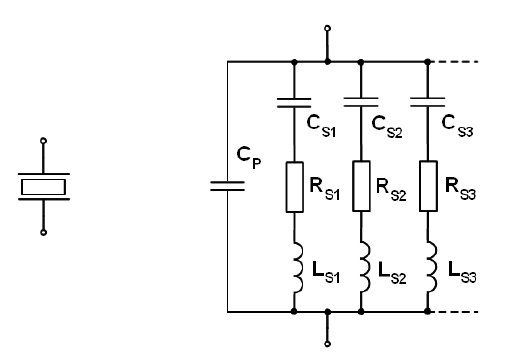
\includegraphics[scale=0.4]{Obrazky/VFT/model_krystal.png}}
		\captionsetup{justification=centering}
		\caption{Schematická značka a náhradný obvodový model krystalu}
	\end{figure}
	
	Prvky $L_{S1}$, $R_{S1}$, $C_{S1}$ -- tvoria sériový rezonančný obvod, ktoré sú dané mechanickými vlastnosťami a určujú jeho základný sériový rezonančný kmitočet. 
	-- Ďalšie sériové rezonančné obvody predstavujú vyššie násobky (harmonické) rezonančného kmitočtu krystalu.\\
	\medskip
	Kapacita $C_p$: 
	\begin{itemize}[label=--]
	%\vspace{-2.5mm}
	\item predstavuje kapacitu elektród a držiaku samotného piezokrystalového rezonátora,
	\item vďaka tejto kapacite vykazuje krystal okrem sériovej rezonancie $f_s$ aj paralelnú rezonanciu $f_p$
	\end{itemize}	 
	
	$C_{ekv}$ -- sériová kombinácia $C_{S1}$ a $C_{p}$\\	 
	\medskip
	-- pre rezonančné kmitočty sériovej a paralelnej rezonancie platia vzťahy (prvá harmonická):
\noindent
\begin{minipage}[t]{0.48\textwidth}
	\begin{equation}
		f_s = \frac{1}{2\pi \sqrt{L_{S1} C_{S1}}}
	\end{equation}
\end{minipage}
\hfill
\begin{minipage}[t]{0.48\textwidth}
	%\vspace{-6mm}
	\begin{equation}
		f_p = \frac{1}{2\pi \sqrt{L_{S1} C_{ekv}}}
		=
		f_s \sqrt{1+\frac{C_{S1}}{C_p}}
	\end{equation}
\end{minipage}
	
	\begin{figure}[H]
		%\vspace{-2mm}
		\makebox[\textwidth]{%
			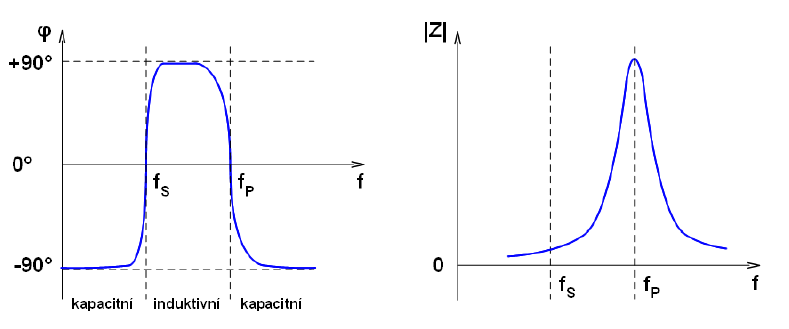
\includegraphics[scale=0.45]{Obrazky/VFT/kmitoctova_zavislost_krystal.png}}
		\captionsetup{justification=centering}
		\caption{Kmitočtová závislosť fáze a modulu impedanci krystalu v okolí prvej harm.}
	\end{figure}
	-- na kmitočtoch $f < f_s$ ma kapacitný charakter\\
	-- na kmitočtoch $f_s < f < f_p$ ma induktívny charakter\\
	-- krystaly sa zapojujú do priečkových štruktúr a vytvárajú vysoko selektívne pásmové~priepuste
	
	
\begin{figure}[H]
	%\vspace{-2mm}
	\makebox[\textwidth]{%
		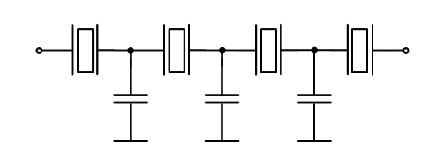
\includegraphics[scale=0.45]{Obrazky/VFT/krystal_prieckove_struktury.png}}
	\captionsetup{justification=centering}
	\caption{Priečkové štruktúry krystalovej pásmovej priepusti}
\end{figure}

\textbf{Piezokeramické filtry:}
\begin{itemize}[label=--]
%\vspace{-2mm}
\item rezonátor je tvorený keramickou dostičkou, ktorá je vyrobená lacnejšie než výbrus z mnohokryštálu kremeňa
\item majú menšiu jakosť než krystalové (vykazujú vyšší útlm v priepustnom pásme)
\end{itemize}

\textbf{Filtry s povrchovou akustickou vlnou (SAW)}
\begin{itemize}[label=--]
%\vspace{-2mm}
\item mechanické kmity sa vytvárajú pomocou vhodných elektromagnetických meničov na povrchu piezoelektrického substrátu
\item elektrický signál prechádza na vstupný elektromechanický menič, ktorý je tvorený elektrodami v tvare hrebeňov naparených na piezoelektrickom substráte
\item elektródy vybudia akustické (mechanické) vlny, ktoré sa po povrchu materiálu šíria k výstupným elektródam rýchlosťou približne akustických vĺn (vo voľnom prostredí)
\item vo výstupnom meniči sú vlny premenené na elektrický signál
\end{itemize}

\begin{figure}[H]
	%\vspace{-2mm}
	\makebox[\textwidth]{%
		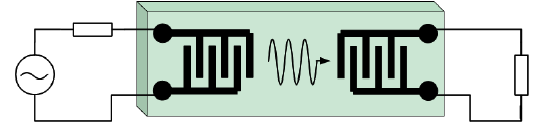
\includegraphics[scale=0.5]{Obrazky/VFT/SAW.png}}
	\captionsetup{justification=centering}
	\caption{Filter s povrchovou akustickou vlnou (SAW)}
\end{figure} 
	
\subsubsection{Směrování a řízení úrovně vf signálu}

{\raggedright \textbf{Wilkinsonov delič:}}
\begin{itemize}[label=--]
%\vspace{-2.5mm}
\item privádzame signál na port 1, pričom výkon je rozdelený na polovice medzi porty 2 a 3 s rovnakou fázou
\item ak používame obvod ako zlučovač privádzame signál na port 2 a 3, na porte 1 je zlúčený signál
\item medzi portmi 2 a 3vzniká izolácia v radoch desiatok dB
\item obvod je úzkopásmovy navrhnutý pre určitý stredný kmitočet
\end{itemize}
\begin{figure}[H]
	%\vspace{-2mm}
	\makebox[\textwidth]{%
		
\includegraphics[scale=0.225]{Obrazky/VFT/willkinson_delic.png}}
	\captionsetup{justification=centering}
	\caption{Wilkinsonov delič} %Wilkinsonov delič/zlučovač v a.) diskretnom prevedení, b.) zo štvrťvlnného úseku vedenia, c.) schématicka značka
\end{figure} 	

{\raggedright \textbf{Hybridný člen:}}
\begin{itemize}[label=--]
%\vspace{-2.5mm}
\item používa sa ako delič/zlučovač výkonu s 90$\degree$ vzájomným fázovým posuvom
\item vo funkcii \textbf{deliča výkonu} privádzame na port 1 signál, ktorý sa rozdelí medzi \mbox{porty 2 a 4}
\item medzi portami 2 a 4 vzniká izolácia a fázový posuv 90\degree
\item port 3 je zakončený $R = Z_0$	
\item pripojením signálu na porty 2 a 4 je možné použiť obvod ako \textbf{zlučovač} s výstupom port~1	
\item šírka pásma podobná Wilkinsonovy, obvod je navrhnutý pre určitý stredný kmitočet
\end{itemize}
\begin{figure}[H]
	%\vspace{-2mm}
	\makebox[\textwidth]{%
		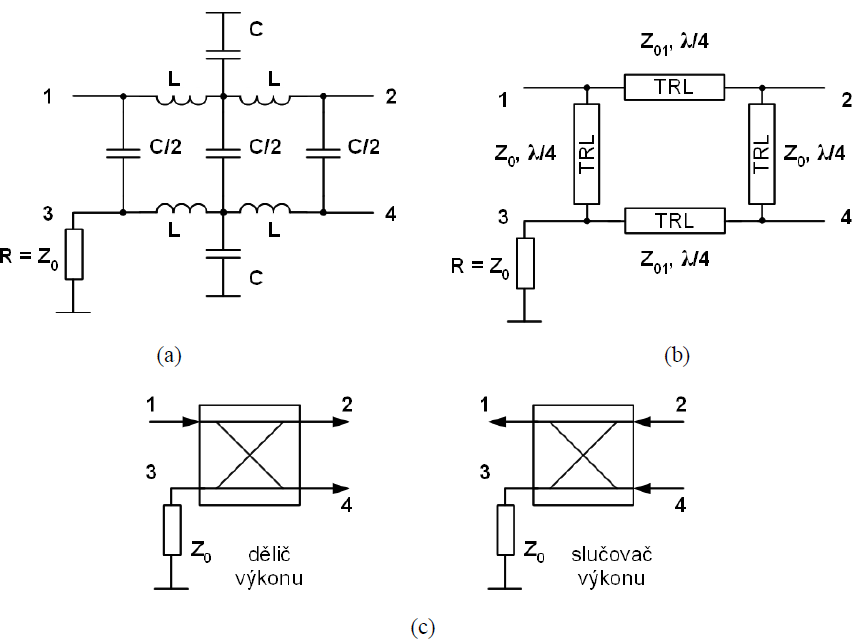
\includegraphics[scale=0.375]{Obrazky/VFT/hybridny_clen.png}}
	\captionsetup{justification=centering}
	\caption{Hybridný člen v a.) diskrétnom prevedení, b.) zo štvrťvlnného úseku vedenia, c.) schématicka značka}
\end{figure} 
\newpage
\textbf{Vysokofrekvenčné prepínače:} \\
\medskip
\textbf{Elektromechanické prepínače:} \\
\medskip 	
\textbf{\small Relé:}
\begin{itemize}[label=--]
	%\vspace{-2.5mm}
		  \item vysokofrekvenčné relé schopné prenášať veľké výkony bez skreslenia
		  \item vyznačujú sa nízkym vloženým útlmom a širokopásmovosťou
		  \item nevýhodou je ich veľkosť, hmotnosť, nízka rýchlosť prepínania
		  \item dajú sa použiť do kmitočtov niekoľko GHz
\end{itemize}

\textbf{\small MEMS:}
\begin{itemize}[label=--]
	%\vspace{-2.5mm}
		  \item založené na mechanickom princípe prepínania vo forme integrovaných obvodov
		  \item veľmi vysoká linearita, malé veľkosti a dosahujú šírky pásma desiatok GHz
\end{itemize}
	
\textbf{Polovodičové prepínače:}
\begin{itemize}[label=--]
	%\vspace{-2.5mm}
		  \item realizované pomocou PIN diód, v integrovaných obvodoch prepínače na báze poľom riadené GaAs FET tranzistory
		  \item vyznačujú sa veľkou rýchlosťou prepínania a vysokou spoľahlivosťou
		  \item majú výkonové obmedzenia
\end{itemize}

\textbf{\small Vlastnosti PIN diódy:}
\begin{itemize}[label=--]
	%\vspace{-2.5mm}
		  \item u PIN diódy je oblasť P od oblasti N izolovaná vrstvou I, ktorá nie je dotovaná žiadnou prímesou a vykazuje iba vlastnú (intrizitnú) vodivosť
		  \item napätie v priamom smere: injekcia nosičov do oblasti I, odpor sa zmenšuje v závislosti na prechádzajúcom prúde 
		  \item dióda pre signál predstavuje nízku impedanciu 	
		  \item napätie v opačnom smere (v závernom smere): odčerpávanie náboja z vrstvy I $\rightarrow$ vytvorí sa oblasť priestorového náboja $\rightarrow$ dióda sa správa ako kondenzátor a predstavuje pre signál vysokú impedanciu
\end{itemize}

		  \begin{figure}[H]
		  	%\vspace{-2mm}
		  	\makebox[\textwidth]{%
		  		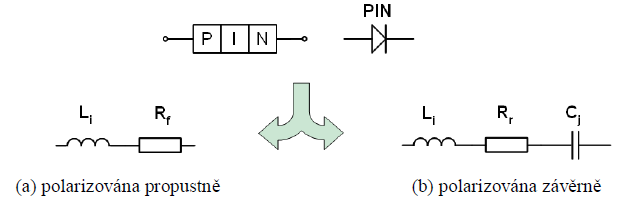
\includegraphics[scale=0.55]{Obrazky/VFT/pin_dioda.png}}
		  	\captionsetup{justification=centering}
		  	\caption{Náhradný obvod PIN diódy}
		  \end{figure} 
		  
		  
\textbf{Atenuátory:}
\begin{itemize}[label=--]
	%\vspace{-2.5mm}
	\item je to útlmový článok, ktorý ma za úlohu vytvoriť v obvode presne definovaný vložený útlm
	\item používajú sa bežne topológie ako $\Pi$ alebo $T$
	\item slúžia na zlepšenie impedančného prispôsobenia a ochranu citlivých častí zariadení pred preťažením
	\item môžu byť pevné alebo nastaviteľné (tvorené pomocou PIN diód)
\end{itemize}

	  \begin{figure}[H]
		%\vspace{-2mm}
		\makebox[\textwidth]{%
			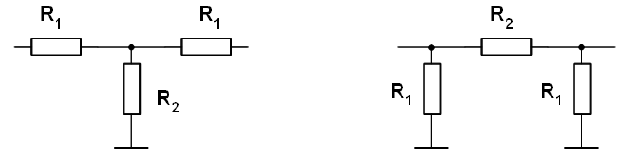
\includegraphics[scale=0.4]{Obrazky/VFT/attenuatory.png}}
		\captionsetup{justification=centering}
		\caption{Topológie atenuátorov T a $\Pi$}
	\end{figure} 
%	\begin{itemize}[label=--]
%		\item paralelný rezonančný obvod je možné použiť na výkonové prispôsobenie generátora k záťaži
%		\item uvažuje sa prípad, keď sú admitancie generátora aj záťaže čisto reálne:
%		\begin{equation}
%			G_S = \frac{1}{R_S}, \qquad G_L = \frac{1}{R_L}
%		\end{equation}
%		\item podmienka výkonového prispôsobenia:
%		\begin{equation}
%			Y_S = Y_L^{*}
%		\end{equation}
%		\item pri čisto reálnych admitanciách platí:
%		\begin{equation}
%			G_S = G_L
%		\end{equation}
%		\item vodivosť generátora sa transformuje:
%		\begin{itemize}[label=$\rightarrow$]
%			\item kapacitným deličom s transformačným pomerom $p_1$
%		\end{itemize}
%		\item vodivosť záťaže sa transformuje:
%		\begin{itemize}[label=$\rightarrow$]
%			\item odbočkou na cievke s transformačným pomerom $p_2$
%		\end{itemize}
%		\item podmienka výkonového prispôsobenia po transformácii:
%		\begin{equation}
%			p_1^2 G_S = p_2^2 G_L
%		\end{equation}
%		\item vhodným nastavením transformačných pomerov $p_1$ a $p_2$ možno dosiahnuť výkonové prispôsobenie
%		\item prispôsobenie platí iba v úzkom okolí rezonančného kmitočtu:
%		\begin{equation}
%			f_0
%		\end{equation}
%		\item ide o úzkopásmový prispôsobovací obvod
%		\item výkonové prispôsobenie nie je ideálne kvôli vlastnej vodivosti rezonátora:
%		\begin{equation}
%			G_0
%		\end{equation}
%		\item výsledná vodivosť zaťaženého obvodu:
%		\begin{equation}
%			G = p_1^2 G_S + G_0 + p_2^2 G_L
%		\end{equation}
%		\item z výslednej vodivosti možno určiť:
%		\begin{itemize}[label=$\rightarrow$]
%			\item činiteľ akosti zaťaženého obvodu $Q$
%			\item účinnosť
%			\item stratový vložný útlm
%		\end{itemize}
%		\item ideálne bezstratové výkonové prispôsobenie by nastalo iba pri:
%		\begin{equation}
%			G_0 = 0
%		\end{equation}
%		\item podmienka $G_0 = 0$ by platila iba pre ideálne bezstratové súčiastky $L$ a $C$
%	\end{itemize}
								
%	
%	Vplyv záťaže na paralelný rezonančný obvod je možné obmedziť 
	\newpage
%	\section{\normalsize Kritérium a kružnice stability. Šumové číslo. Šum atenuátoru a zesilovače. Dynamický rozsah DR a SFDR. Linearizovaný a velkosignálový zesilovač. Nízkošumový zesilovač, šumové přizpůsobení.}
	\chapter{Otázka VFT 2.}
	\subsubsection{Stabilita zosilňovača}

	\begin{itemize}[label=--]
	%\vspace{-2mm}
	\item pri nestabilite tranzistora dochádza ku vzniku netlmených kmitov --> stáva sa z neho oscilátor
	\item k rozkmitaniu dochádza použitím určitej impedancie na vstup alebo výstup tranzistora
	\item vyšetrenie stability: zistiť pre aké impedancie nastáva nestabilita 
	\end{itemize}
	
	  \begin{figure}[H]
		%\vspace{-2mm}
		\makebox[\textwidth]{%
			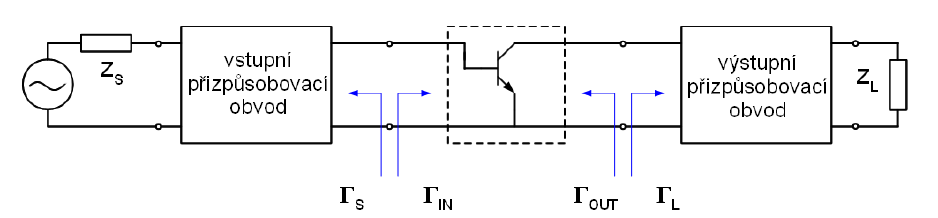
\includegraphics[scale=0.4]{Obrazky/VFT/tranzistor.png}}
		\captionsetup{justification=centering}
		\caption{Tranzistor (zosilňovač)}
	\end{figure} 
	
	\begin{itemize}[label=]
	\item $\Gamma_S$ -- závisí na impedancii generátora, ktorá je transformovaná vstupným prispôsobovacím obvodom\\
	\item $\Gamma_L$ -- závisí na impedancii záťaže, ktorá je transformovaná výstupným prispôsobovacím obvodom\\
	\item $\Gamma_{IN}$ -- závisí na činiteli odrazu $\Gamma_L$ a na matici s - parametrov tranzistora \\
	\item $\Gamma_{OUT}$ -- závisí na činiteli odrazu $\Gamma_S$ a na matici s - parametrov tranzistorov\\
	\end{itemize}
	
	\textbf{Absolútna stabilita}\\
	%\vspace{-1mm}
	-- tranzistor je na danej frekvencii absolútne stabilný, ak platí:\\
	%\vspace{-1mm}	
	\begin{tcolorbox}[
		colback=blue!5,
		colframe=blue,
		boxrule=0.8pt,
		arc=2mm
			]
		\centering
		$\abs{\Gamma_{IN}} < 1$ a zároveň $\abs{\Gamma_{OUT}} < 1$
		\textbf{ pre všetky impedancie} pripojené na vstup alebo výstup tranzistora
		(pričom $\abs{\Gamma_S}<1$ a $\abs{\Gamma_L}<1$).
	\end{tcolorbox}
	%\vspace{1mm}	
	{\raggedright \textbf{Podmienečná stabilita}}\\
	- tranzistor je podmienečne stabilný (potencionálne nestabilný) v prípade, že platí:\\
	%\vspace{-1mm}
	
	\begin{tcolorbox}[
		colback=blue!5,
		colframe=blue,
		boxrule=0.8pt,
		arc=2mm
		]
		\centering
		$\abs{\Gamma_{IN}} < 1$ a zároveň $\abs{\Gamma_{OUT}} < 1$
		\textbf{iba pre niektoré impedancie} pripojené na vstup alebo výstup tranzistora
		(pričom $\abs{\Gamma_S}<1$ a $\abs{\Gamma_L}<1$).
	\end{tcolorbox}
	
%	$\abs{\Gamma_{IN}} < 1$ a zároveň $\abs{\Gamma_{OUT}} < 1$ \textbf{iba pre niektoré impedancie} pripojené na vstup alebo výstup tranzistora (pričom $\abs{\Gamma_S}<1$ a $\abs{\Gamma_L}<1$).\\
	%\vspace{0mm}
	- stabilitu tranzistora je možné riešiť graficky v Smithovom diagrame pomocou kružníc stability alebo analyticky pomocou kritérií\\
	%\vspace{1mm}
	{\raggedright \textbf{Kružnice stability}}\\
	%\vspace{1mm}	
	- kružnice vyznačujú hranicu medzi stabilnou a nestabilnou oblasťou vo Smithovom diagrame\\
	- ak pripojíme ku vstupu (resp. výstupu) tranzistora záťaž s činiteľom odrazu z nestabilnej oblasti, bude tranzistor na výstupe (resp. vstupe kmitať)\\
	- činiteľ odrazu na vstupu tranzistora $\Gamma_{IN}$ závisí na záťaži na jeho výstupu $\Gamma_L$\\
	- činiteľ odrazu na výstupu tranzistora $\Gamma_{OUT}$ závisí na záťaži na jeho vstupu $\Gamma_S$\\
	- záťaž pripojená na výstup tranzistora ovplyvňuje stabilitu jeho vstupu a naopak \\
	\newpage
	{\raggedright \textbf{Kružnice stability pre výstup} (zobrazuje $\Gamma_L$)}\\
	- predstavuje hranicu medzi stabilnou a nestabilnou oblasťou výstupných činiteľov odrazu $\Gamma_L$, na ktorej $\abs{\Gamma_{IN}} = 1$ $\rightarrow$ vstup tranzistora je na medzi stability \\
	- pripojením na výstup tranzistora impedanciu z nestabilnej oblasti spôsobí nestabilitu na vstupe\\
	 
	 \begin{figure}[H]
		%\vspace{-2mm}
		\makebox[\textwidth]{%
			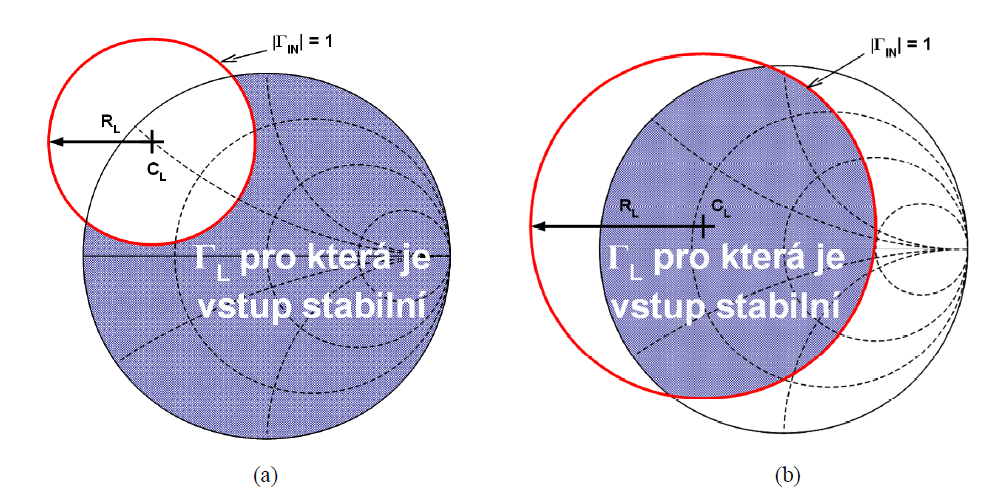
\includegraphics[scale=0.4]{Obrazky/VFT/kruznica_stability_vystup.png}}
		\captionsetup{justification=centering}
		\caption{Kružnice stability pre výstup $\Gamma_L$ za predpokladu $\abs{S_{11}} < 1$}
	\end{figure} 
	
	- Platí, ak $\abs{S_{11}} < 1$ $\rightarrow$ oblasť kružnice stability, v ktorej leží stred Smithova diagramu \textbf{stabilná oblasť} a mimo kružnice je nestabilná oblasť.\\
	- Ak stred Smithova diagramu, leží mimo kružnice tak je to naopak (vonkajšia oblasť stabilná, vnútorná nestabilná)\\
	%\vspace{1mm}
	{\raggedright \textbf{Kružnice stability pre vstup} (zobrazuje $\Gamma_S$)}\\
	- predstavuje hranicu medzi stabilnou a nestabilnou oblasťou vstupných činiteľov odrazu $\Gamma_S$, na ktorej $\abs{\Gamma_{OUT}} = 1$ $\rightarrow$ výstup tranzistora je na medzi stability \\
	- pripojením na vstup tranzistora impedanciu z nestabilnej oblasti spôsobí nestabilitu na výstupe
	
	\begin{figure}[H]
		%\vspace{-2mm}
		\makebox[\textwidth]{%
			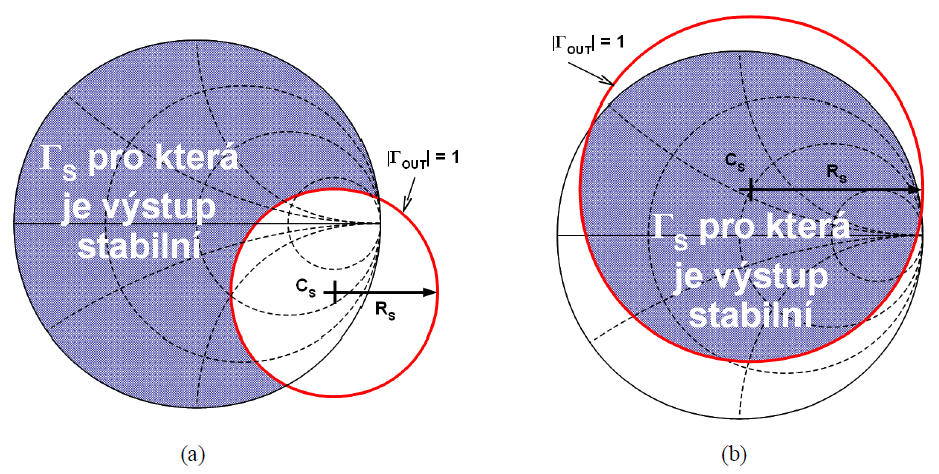
\includegraphics[scale=0.4]{Obrazky/VFT/kruznica_stability_vstup.png}}
		\captionsetup{justification=centering}
		\caption{Kružnice stability pre výstup $\Gamma_L$ za predpokladu $\abs{S_{11}} < 1$}
	\end{figure} 
	
	- platí, ak $\abs{S_{22}} < 1$ --> oblasť kružnice stability, v ktorej leží stred Smithova diagramu \textbf{stabilná oblasť} a mimo kružnice je nestabilná oblasť.\\
	- ak stred Smithova diagramu, leží mimo kružnice tak je to naopak\\
	%\vspace{1mm}
	{\raggedright \textbf{Analytické kritéria stability}}
	 
	 \textbf{Kritérium stability 1:} tranzistor je absolútne stabilný v prípade, že platí: $K > 1$ a zároveň $\abs{\Delta} < 1$ \\
	
	 \textbf{Kritérium stability 2:}
	- tranzistor je absolútne stabilný v prípade, že platí: $K > 1$ a zároveň $B_1 > 0$\\
	- kritéria su matematicky ekvivalentné a je možné použiť ktorékoľvek z nich\\
	
	Z podmienok pre stabilitu sú definované tieto parametre:\\
		-- determinant matice s-parametrov $\Delta$\\
		-- Rolletov činiteľ stability\\
		-- parameter $B_1$\\
	%\vspace{2.5mm}
	Širokopásmová stabilizácia tranzistora\\
	-- dá sa to pomocou \\
		$\rightarrow$ rezistívnej záťaže \\
		$\rightarrow$ zápornej spätnej väzby \\
	-- obe spôsoby majú za následok zníženie zisku a zvýšenie šumového čísla zosilňovača \\
	
	\subsubsection{Šum v aktívnych a pasívnych obvodoch}
	%\vspace{-2mm}
	-- tepelný šum vzniká na reálnej časti každej impedancie vplyvom tepelného pohybu částic \\
	-- vykazuje konšt. spektrálnu hustotu výkonu (nezávisí na frekvencii) \\
	-- vyskytuje sa v pasívnych a aktívnych súčiastkach \\
	-- pre šumový výkon platí:\\
	\begin{equation}
		P_N = k T B
	\end{equation}
	kde k -- Boltzmanova konšt., T -- teplota (K), B - šumová šírka pásma\\
	Z toho vyplýva:\\
	-- tepelný šum nezávisí na pracovnej frekvencii obvodu, ale na šírke pásma --> úzkopásmové obvody produkujú menej šumu\\
	-- s klesajúcou teplotou klesá aj výkon tepelného šumu (chladnejšie súčiastky -- menej šumu)\\
	%\vspace{1mm}
	{\raggedright \textbf{Vystreľovaný šum:}}\\
	-- vzniká pri prechode nosičov náboja PN prechodom, pri prechode jednosmerného prúdu PN prechodom \\
	-- vyskytuje sa u trazistorov a diod \\
	-- vykazuje konštantu spektrálnu hustotu výkonu \\
	%\vspace{1mm}
	{\raggedright \textbf{Šum 1/f:}}\\
	-- vzniká v dôsledku poruch krystalickej mriežky polovodičov a vplyvom nečistôt v polovodiči \\
	-- spektrálna hustota výkonu klesá s rastúcim kmitočtom\\
	{\raggedright \textbf{Šumová šírka pásma:}}\\
	-- aktívne aj pasívne obvody vykazujú určité selektívne vlastnosti \\
	-- ak na vstupe je šumový signál s konšt. spektrálnou hustotou výkonu $\rightarrow$ selektívny šum \\
	-- spektrálna hustota signálu má na $f_0$
	
	\begin{figure}[H]
		%\vspace{-2mm}
		\makebox[\textwidth]{%
			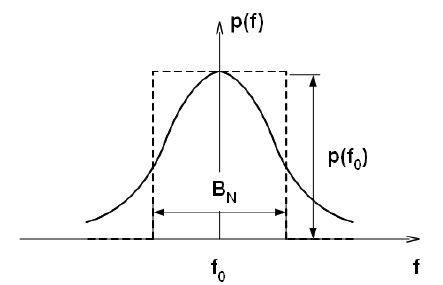
\includegraphics[scale=0.4]{Obrazky/VFT/sumova_sirka_pasma_obvodu.png}}
		\captionsetup{justification=centering}
		\caption{Šumová šírka pásma obvodu}
	\end{figure} 
	
	-- šumová šírka pásma $B_N$ sa určí na základe rovnosti celkového šumového výkonu na výstupe a ekvivalentného šumového výkonu, ktorý by sme získali na výstupe selektívneho obvodu s ideálnou obdĺžnikovou prenosovou charakteristikou \\
	-- musí platiť, že plocha pod krivkou $p(f)$ sa rovná ploche obdĺžnika so stranami $p(f_0)$ a $B_N$\\
	\newpage
	{\raggedright \textbf{Ekvivalentná šumová a teplota a šumové číslo:}}\\
	-- zdroj bieleho šumu môže byť nahradený šumiacim rezistorom s ekvivalentnou šumovou teplotou \\
	\begin{equation}
		T_e = \frac{P_N}{kB}
	\end{equation}
	kde $B$ je šumová šírka pásma\\
	-- zdroj bieleho šumu je možné nahradiť rezistorom o teplote $T_e$, ktorý vyprodukuje ekvivalentný šumový výkon $P_N$

	\begin{figure}[H]
	%\vspace{-2mm}
	\makebox[\textwidth]{%
		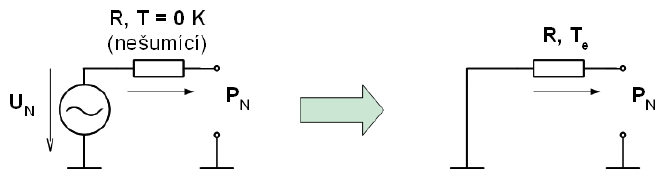
\includegraphics[scale=0.5]{Obrazky/VFT/zdroj_sumu.png}}
	\captionsetup{justification=centering}
	\caption{Zdroj tepelného (bieleho) šumu a jeho ekvivalentný obvodový model}
	\end{figure} 	
	
	{\raggedright \textbf{Šumové číslo aktívneho obvodu:}}\\
	-- šumové číslo $F$ charakterizuje šumové vlastnosti samotného aktívneho obvodu\\
	-- je mierkou toho, ako samotný obvod prispieva k celkovému výstupnému výkonu šumu\\
	-- šumové číslo je vždy $F>1$, resp. v dB $F(\text{dB})>0\text{dB}$\\
	-- vzťahuje sa k referenčnej teplote $T_0 = 290 \text{ K}$\\
	%\vspace{1mm}
	{\raggedright \textbf{Šumové číslo pasívneho obvodu:}}\\
	-- šumové číslo v dB je rovné vloženému útlmu pasívneho obvodu v dB (za predpokladu $T = T_0$)\\
	%\vspace{1mm}
	Šumové číslo pasívneho obvodu o fyzickej teplote $T$ je: \\
	\begin{equation}
		%\vspace{-1mm}
		F = 1 + (L-1)\frac{T}{T_0}
	\end{equation}
		%\vspace{2mm}
	-- pri teplote $T = T_0 = 290 \text{ K}$ sa vzťah zjednoduší $\rightarrow$ F = L \\
	%\vspace{1mm}
	{\raggedright \textbf{Definícia šumového čísla pomocou výkonu signálu a šumu:}}
	\begin{equation}
		F = \frac{P_S^{IN}/P_N^{IN}}{P_S^{OUT}/P_N^{OUT}} = \frac{SNR^{IN}}{SNR^{OUT}} 
	%\vspace*{1mm}
	\end{equation}
	{\raggedright \textbf{Šumové číslo kaskádne riadených obvodov:}} \\
		- každý z blokov prispieva vlastným šumom \\
		\begin{figure}[H]
		%\vspace{-2mm}
		\makebox[\textwidth]{%
			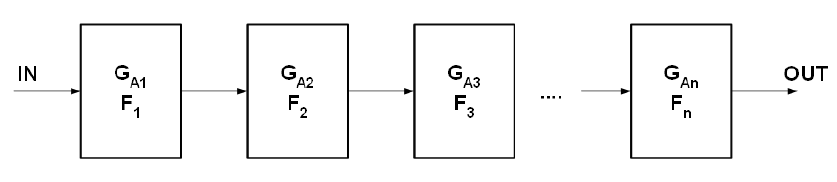
\includegraphics[scale=0.375]{Obrazky/VFT/kaskada_blok_obvodov_F.png}}
		\captionsetup{justification=centering}
		\caption{Kaskáda blokov}
		\end{figure} 
	%\vspace{-1mm}
		{\raggedright \textbf{Friisov vzťah:}}
		%\vspace{2mm}
		\begin{equation}
			F = F_1 + \frac{F_2 - 1}{G_{A1}}+\frac{F_3 - 1}{G_{A1} G_{A2}}+\frac{F_4 - 1}{G_{A1} G_{A2} G_{A3}}+\dots
		%\vspace{1mm}
		\end{equation}
		-- pomocou Friisovho vzťahu je možné vypočítať výsledné šumové číslo kaskády\\
		-- Friisov vzťah platí za podmienky výkonového prispôsobenia jednotlivých stupňov kaskády \\
		-- celkové šumové číslo bude závisieť na poradí jednotlivých blokov v kaskáde\\
		
		\textbf{Zoradenie obvodových blokov kaskády pre minimálne šumové číslo}: \\
		-- ako prvý stupeň sa zaradzuje ten blok, ktorý ma nízke šumové číslo a vysoký zisk \\
		
	\subsubsection{Dynamický rozsah DR zosilňovača}
	%\vspace*{-2mm}
	- pri zvyšovaní vstupnej výkonovej úrovne, narastá výstupná výkonová úroveň úmerne zisku zosilňovača (v ideálnom prípade do nekonečna) \\
	- reálny aktívny prvok má obmedzený výstupný výkon, ktorý je schopný dodať do záťaže, dochádza k odklonu od ideálnej lineárnej závislosti \\
	
	\begin{figure}[H]
		%\vspace{-2mm}
		\makebox[\textwidth]{%
			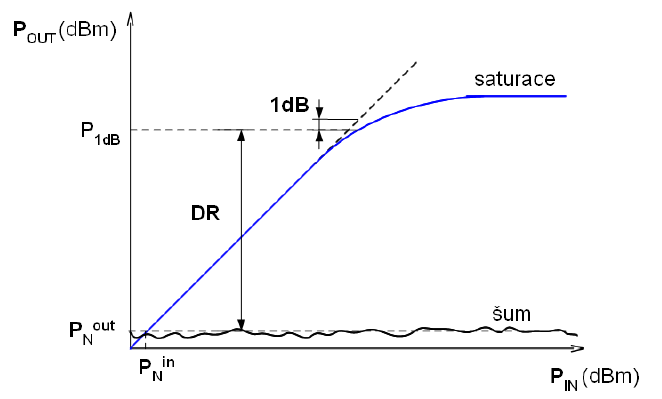
\includegraphics[scale=0.4]{Obrazky/VFT/dynamicky_rozsah.png}}
		\captionsetup{justification=centering}
		\caption{Dynamický rozsah}
	\end{figure} 
	
	Dynamický rozsah zosilňovača je definovaný ako rozdiel výstupných výkonových úrovni:
	\begin{equation}
		DR\text{(dB)} = P_{\text{1dB}} - P_N^{\text{OUT}} (\text{dBm}) 
	\end{equation}
	
	$P_{\text{1dB}}$ - výstupný výkon v bode jednodecibelovej kompresie zisku,\\
	$P_N^{\text{OUT}}$ - výstupná výkonová úroveň šumovej hladiny \\
	%\vspace{2mm}
	\textbf{Bod jednodecibelovej kompresie} $\mathbf{P_{\text{1dB}}}$\\
	-- bod jednodecibelovej kompresie $P_{\text{1dB}}$ je výstupný výkon, pri ktorom nastáva pokles zisku zosilňovača o 1 dB \\
	-- pri ďalšom zvyšovaní vstupného výkonu zisk ďalej klesá až dôjde k saturácii aktívneho prvku -- tento bod považujeme za hranicu linearity zosilňovača\\
	%\vspace{2mm}
	\textbf{Dynamický rozsah bez intermodulačného skreslenia (SFDR)}\\
	-- SFDR určuje maximálny dynamický rozsah v ktorom sú intermodulačné produkty ešte pod hladinou šumu -- nezasahujú do užitočného signálu\\
	-- je daný vzdialenosťou (na ose $P_{OUT}$) od bodu, kedy začnú IM3 (intermodulačné produkty 3. radu) vystupovať z šumu, do priesečníka s charakteristikou užitočného signálu \\ 
	%% dopisať IM3 a intermodulačné skreslenie
	
	\begin{figure}[H]
	%\vspace{-2mm}
	\makebox[\textwidth]{%
		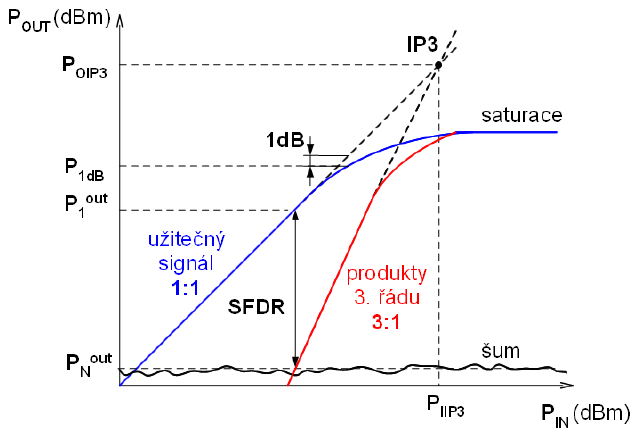
\includegraphics[scale=0.4]{Obrazky/VFT/SFDR_char.png}}
	\captionsetup{justification=centering}
	\caption{Bod zahradenia zosilňovača}
	\end{figure} 
	
	\newpage
	\subsubsection{Linearizovaný a veľkosignálový zosilňovač}
	
	\textbf{Linearizovaný zosilňovač}
	\begin{itemize}[label=--]
	%\vspace{-2mm}
		\item ide o zosilňovač, ktorý pracuje s malým signálom vo veľmi úzkom okolí pracovného bodu (jednosmerného) a neprejavuje sa u nich nelinearita prevodných charakteristík tranzistora 
		\item považuje sa za lineárny dvojbran
		\item k návrhu zosilňovača používame s-parametry
	\end{itemize}
	\medskip
	
	\textbf{Veľkosignálový zosilňovač}
	\begin{itemize}[label=--]
	%\vspace{-2mm}
		\item slúži na zosilnenie vf. signálov s vysokým výkonom
		\item používa sa vo výkonových stupňoch vysielačov
		\item cieľom návrhu je dosiahnuť vysoký výstupný výkon a vysokú účinnosť
		\item vyššia účinnosť je dosahovaná za cenu väčšieho nelineárneho skreslenia
		\item dôležitými parametrami sú výstupný výkon, účinnosť a linearita
		\item univerzálnou metódou návrhu je load-pull technika využívajúca činitele odrazu $\Gamma_{SP}$ a $\Gamma_{LP}$
	\end{itemize}
	
	\textbf{Nízkošumový zosilňovač}
	\begin{itemize}[label=--]
	%\vspace{-2mm}
		\item slúži na zosilnenie veľmi slabých vf. signálov pri minimálnom pridaní vlastného šumu
		\item cieľom návrhu nízkošumového zosilňovača je dosiahnuť nízke šumové číslo a vysokú hodnotu zisku
		\item používajú sa tranzistory s veľmi malým $S_{12}$ a veľmi dobrými šumovými parametrami
		\item používa sa najmä na vstupoch prijímačov
		\item dôležitými parametrami sú šumové číslo, zisk a stabilita
		\item vstup býva prispôsobený pre dosiahnutie minimálneho šumového čísla
	\end{itemize}

	{\raggedright \textbf{Šumové prispôsobenie tranzistorov}}
	\begin{itemize}[label=--] 
	\item pri návrhu nízkošumového zosilňovača (LNA) vstup tranzistora prispôsobujeme na činiteľ odrazu $\Gamma_{opt}$, aby vykazoval šumové číslo $F_{min}$
	\item parametre $F_{min}$, $\Gamma_{opt}$ sú udávane výrobcom v datasheete
	\end{itemize}

	
%	\section{\normalsize  Parametry směšovačů. Zpětnovazební oscilátor, podmínka oscilací. Tříbodová zapojení, přeladitelnost. Vlastnosti oscilátorů. Typy PLL syntezátoru, princip DDS, jejich spektrální vlastnosti.}
	\chapter{Otázka VFT 3.}
 	
	\textbf{Zmiešavač}
	%\vspace{-2mm} 
	\begin{itemize}[label=--] 
	\item nelineárny obvod so dvoma vstupmi a jedným výstupom, ktorý generuje spektrum dané súčtom alebo rozdielom dvoch vstupných kmitočtov a ich násobkov
	\item vstupné porty sa označujú: 
			\begin{itemize}[label=$\rightarrow$]
			%\vspace{-3.5mm} 
			\item RF (vstup vf. signálu - Radio Frequency), 
			\item LO (vstup signálu miestneho oscilátoru - Local Oscillator)
			\end{itemize}
	\item výstupný port je označený:
			\begin{itemize}[label=--]
				%\vspace{-3.5mm} 
			\item IF (medzifrekvencie - Intermediate Frequency)
			\end{itemize}
	\end{itemize}
	
	\begin{figure}[H]
		%\vspace{-2mm}
		\makebox[\textwidth]{%
			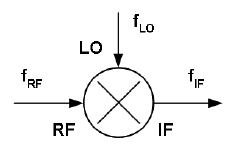
\includegraphics[scale=0.5]{Obrazky/VFT/smesovac.png}}
		\captionsetup{justification=centering}
		\caption{Zmiešavač}
	\end{figure} 
	
	\begin{itemize}[label=--] 
	\item základom zmiešavača je nelineárny prvok (dióda, tranzistor), ktorého nelinearita umožňuje vznik nových spektrálnych zložiek (produkty zmiešavača), ktoré nie su zahrnuté vo vstupných signáloch
	\item signál z lokálneho oscilátora LO musí mať dostatočné vysokú úroveň, aby vyvolal nelineárne správanie obvodu a umožnil vznik produktov zmiešavača
	\item spektrum na výstupe je dané: $f_{IF} = m f_{RF} + n f_{LO}$ 
	(m, n - celé čísla)
	\end{itemize}
	
	\textbf{Down-konvertory} - využívajú rozdielového kmitočtu signálu RF a LO\\
	$f_{IF} = f_{RF} - f_{LO}$ alebo $f_{IF} = f_{LO} - f_{RF}$\\
	-- výsledkom je kmitočet $f_{IF}$ nižší než $f_{RF}$\\
	%\vspace{1.5mm}
	\textbf{Up-konvertory} - využíva súčtového kmitočtu signálu RF a LO\\
	$f_{IF} = f_{RF} + f_{LO}$ \\
	-- výsledkom je kmitočet $f_{IF}$ vyšší než $f_{RF}$ \\
	%\vspace{1.5mm}	
	\textbf{Parametre zmiešavača:}
	\begin{itemize}[label=--]
	%\vspace{-2mm}
	\item konverzné straty $L_C$ alebo konverzný zisk $G_C$ 
	\item šumové číslo 
	\item dynamický rozsah (IP3, $P_{\text{1dB}}$)
	\item izolácia medzi porty 
	\end{itemize}
	
	{\raggedright \textbf{Konverzné straty $L_C$ alebo konverzný zisk $G_C$}}\\
	- konverzné straty sú parametre pasívneho zmiešavača a vyjadrujú pomer medzi výkonom dostupným na vstupe $P_{RF}$ a výkonom na výstupe (na medzifrekvencii) $P_{IF}$\\
	%\vspace{2mm}
	Konverzné straty sú dané vzťahom:
	\begin{equation}
		L_c (\text{dB}) = 10\log \left(\frac{P_{RF}}{P_{IF}}\right)
	\end{equation}
	
	V prípade aktívneho směšovača je to konverzný zisk:
	\begin{equation}
		G_c (\text{dB}) = 10 \log \left(\frac{P_{IF}}{P_{RF}}\right)
	\end{equation}
	
	\textbf{Konverzné straty}: -- je to útlm, ktorý vznikne pri konverzii signálu z RF na IF (mixér vytvára signál s nižším výkonom než signál na vstupe RF)\\
	\medskip
	\textbf{Konverzný zisk}: -- vyjadruje, že úroveň výstupného IF signál je väčšia než na RF vstupe o zisk $G_c$ (aktívne mixéry)\\
	%\vspace{2mm}
	{\textbf{Šumové číslo}}\\
	\begin{itemize}[label=--]
	%\vspace{-2mm}
	\item šum môže prenikať cestou užitočného signálu 
	\item jednokanálový šum, ale aj cestou zrkadlového signálu (nežiadúci signál na zrkadlovom kmitočte, ktorý vzniká pri miešaní signálu)  
	\item šum na druhom kanále
	\end{itemize}
	
	- rozlišuje sa jednokanálové šumové číslo $F_{SSB}$ a dvojkanálové šumové číslo $F_{DSB}$, platí: $F_{DSB} = 2F_{SSB}$ (dvojnásobný šumový výkon).\\
	\newpage
	{\raggedright \textbf{Dynamický rozsah}
	\begin{figure}[H]
		%\vspace{-2mm}
		\makebox[\textwidth]{%
			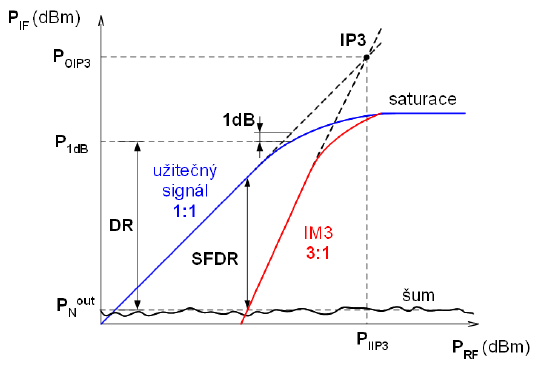
\includegraphics[scale=0.4]{Obrazky/VFT/dynamicky_rozsah_smesovac.png}}
		\captionsetup{justification=centering}
		\caption{Dynamický rozsah a bod zahradení zmiešavača}
	\end{figure} 	
	
	\begin{itemize}[label=--]
		\item dynamický rozsah určuje oblasť lineárnej činnosti zmiešavača
		\item pri veľkých vstupných signáloch dochádza k nelineárnemu skresleniu a saturácii
		\item pri súčasnom spracovaní viacerých signálov vzniká intermodulačné skreslenie
		\item dynamický rozsah charakterizujú parametre:
		\begin{itemize}[label=$\rightarrow$]
			%\vspace{-3mm}
			\item bod jednodecibelovej kompresie $P_{1\mathrm{dB}}$
			\item bod zrazenia tretieho rádu $IP3$
		\end{itemize}
		%\vspace{-2mm}
		\item horná hranica dynamického rozsahu je daná kompresiou zosilnenia o $1\,\mathrm{dB}$
		\item dolná hranica je určená úrovňou šumu
		\item pomocou bodu $IP3$ možno určiť dynamický rozsah bez intermodulačného skreslenia 3. rádu $SFDR$
	\end{itemize}
	
	{\raggedright \textbf{Izolácia portov}}
		\begin{itemize}[label=--]
			\item vzájomná izolácia portov zmiešavača je daná pomerom výkonov signálov rovnakého kmitočtu na dvoch rôznych portoch
			\item najčastejšie sa uvádza v decibeloch
			\item charakterizuje nežiaduce prenikanie signálu medzi jednotlivými bránami
			\item dôležité dosiahnuť vysokú izoláciu LO -- IF - zabránenie prenikaniu signálu z LO na výstup
		\end{itemize}

		\begin{figure}[H]
		%\vspace{-2mm}
		\makebox[\textwidth]{%
			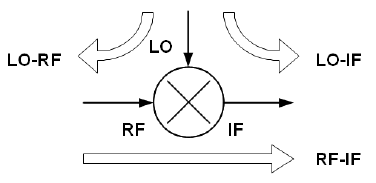
\includegraphics[scale=0.4]{Obrazky/VFT/izolacia_smesovaca.png}}
		\captionsetup{justification=centering}
		\caption{Izolácia portov zmiešovača}
	\end{figure} 
	
	\subsubsection{Spätnoväzobné oscilátory}
	\begin{figure}[H]
		%\vspace{-2mm}
		\makebox[\textwidth]{%
			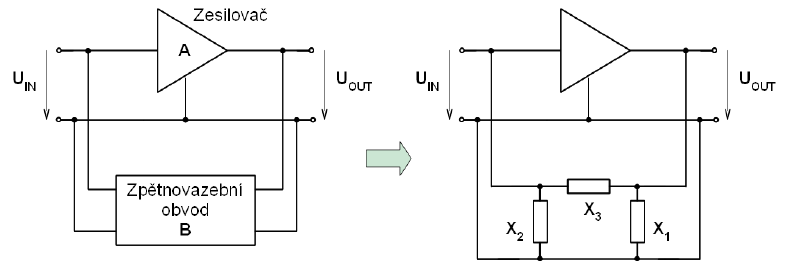
\includegraphics[scale=0.5]{Obrazky/VFT/zosilovac_so_spatnou_vazbou.png}}
		\captionsetup{justification=centering}
		\caption{Zosilňovač so spätnou väzbou}
	\end{figure} 
	
	
	\begin{itemize}[label=--]
		\item na oscilátor je možné pozerať ako na zosilňovač s kladnou spätnou väzbou
		\item oscilátor pozostáva zo zosilňovača s prenosom \textbf{A} a spätnoväzobného obvodu s prenosom~\textbf{B} 
		\item podmienkou vzniku oscilácií je splnenie Barkhausenovej podmienky: $1 -B\cdot A = 0$
		\item pri \textbf{neinvertujúcom zosilňovači} ($\varphi_A=0$) musí spätnoväzobný obvod vytvoriť fázový posun $\varphi_B=0$ (alebo násobok $2\pi$), reaktancie $X_2$ a $X_3$ majú rovnaký charakter, $X_1$ má opačný charakter 
		\item pri \textbf{invertujúcom zosilňovači} ($\varphi_A=\pi$) musí spätnoväzobný obvod vytvoriť fázový posun $\varphi_B=\pi$, reaktancie $X_1$ a $X_2$ majú rovnaký charakter, $X_3$ má opačný charakter 
	\end{itemize}
	
\begin{tcolorbox}[
	colback=blue!5,
	colframe=blue,
	boxrule=0.8pt,
	arc=2mm
	]
	\textbf{Amplitúdová podmienka:}
	\[
	B\cdot A = 1
	\]
	
	\textbf{Fázová podmienka:}
	\[
	\varphi_B + \varphi_A = 0 + k\cdot 2\pi
	\]
\end{tcolorbox}
	
	-- celkový fázový posun musí byť nulový (alebo násobok $\pi$)
	
	\subsubsection{Trojbodové zapojenia}
	
	Základné typy sú: \\
	\begin{itemize}[label=--]
	%\vspace{-4mm}
	\item Hartleyov oscilátor (kapacitný)
	\item Colpittsov oscilátor (induktívny)
	\item Clappov oscilátor
	\end{itemize}
					  
	{\raggedright\textbf{Hartleyov oscilátor:}}
	\begin{figure}[H]
		%\vspace{-2mm}
		\makebox[\textwidth]{%
			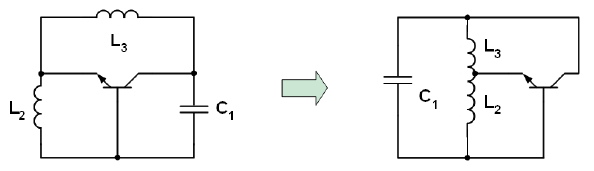
\includegraphics[scale=0.5]{Obrazky/VFT/hartleyov_oscilator.png}}
		\captionsetup{justification=centering}
		\caption{Hartleyov oscilátor}
		%\vspace{-2mm}
	\end{figure} 
	-- veľkosť prenosu spätnej väzby B je daná pomerom $L_2$ a $L_3$\\
	-- polohou odbočky je možné meniť veľkosť spätnej väzby\\
	\begin{equation}
		\omega_0 = \frac{1}{\sqrt{C_1 (L_3 + L_2)}}
	\end{equation}
	
		{\raggedright\textbf{Colpittsov oscilátor:}}
	\begin{figure}[H]
		%\vspace{-2mm}
		\makebox[\textwidth]{%
			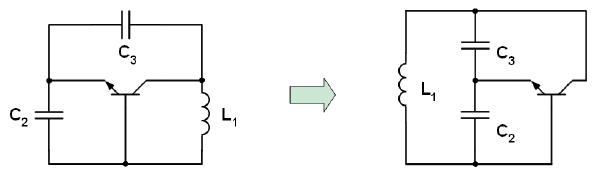
\includegraphics[scale=0.5]{Obrazky/VFT/colpitts_oscilator.png}}
		\captionsetup{justification=centering}
		\caption{Hartleyov oscilátor}
	\end{figure} 
	
	-- veľkosť spätnej väzby sa v tomto prípade nastavuje pomerom kapacít v deliči $C_2$, $C_3$ 

	\begin{equation}
		\omega_0 = \frac{1}{\sqrt{L_1 \left(\frac{C_3 C_2}{C_3 + C_2}\right)}}
	\end{equation}
	
	\newpage
	\textbf{Clappov oscilátor:}
	\begin{figure}[H]
		%\vspace{-2mm}
		\makebox[\textwidth]{%
			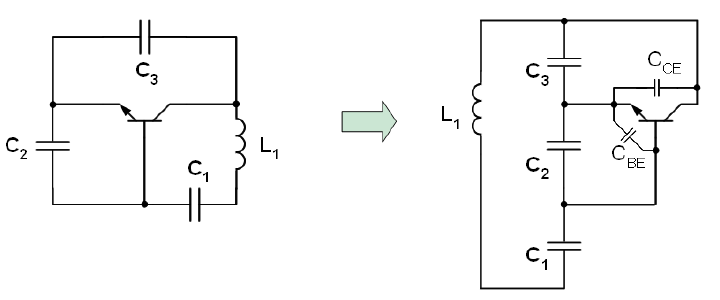
\includegraphics[scale=0.4]{Obrazky/VFT/clappov_oscilator.png}}
		\captionsetup{justification=centering}
		\caption{Clappov oscilátor}
	\end{figure}
	\begin{itemize}[label=--]
	\item modifikácia Clopittsa zmenšuje vplyv medzielektódových kapacít tranzistora na oscilačnom kmitočte
	\item rezonančný kmitočet takmer nezávisí na $C_2$ a $C_3$
	\item výsledná kapacita obvodu je približne rovná $C_1$
	\end{itemize}
	\begin{equation}
		\omega_0 \cong \frac{1}{\sqrt{L_1 C_1}}
	\end{equation}
	
	\textbf{Preladiteľnosť oscilátorov}
	\begin{itemize}[label=--]
	\item zmenu rezonančného kmitočtu LC obvodu je možné previesť zmenou indukčnosti alebo zmenou kapacity
	\item v oscilátoroch sa používajú kapacitné diódy (varikapy), u ktorých je možné meniť ich kapacitu pomocou záverného napätia 
	\item kapacitná dióda musí byť zapojená v závernom smere, v ktorom vykazuje závislosť kapacity $C_d$ prechodu PN na veľkosti priloženého napätia $U_R$
	\end{itemize}

	\begin{figure}[H]
		%\vspace{-2mm}
		\makebox[\textwidth]{%
			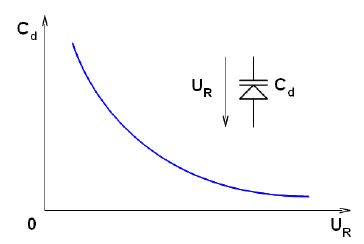
\includegraphics[scale=0.4]{Obrazky/VFT/varikap.png}}
		\captionsetup{justification=centering}
		\caption{Schematická značka a závislosť kapacity na napätiu varikapu}
	\end{figure}
	%\vspace{-2mm}
	-- varianta s 1 diódou sa používa pre: malé striedavé vf. signály (obr. \ref{lad:dioda}.a)\\
	-- variant s 2 diódami sa používa pre: väčšie striedavé vf. signály (obr. \ref{lad:dioda}.b)
	
		\begin{figure}[H]
		%\vspace{-2mm}
		\makebox[\textwidth]{%
			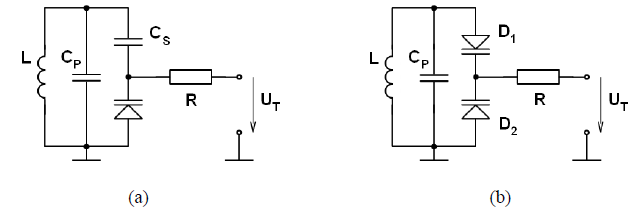
\includegraphics[scale=0.55]{Obrazky/VFT/laditelnost_rezon_obvodov.png}}
		\captionsetup{justification=centering}
		\caption{Paralelný rezonančný obvod ladený kapacitnou diódou}
		\label{lad:dioda}
	\end{figure}
	
	\subsubsection{Vlastnosti krystalových oscilátorov}
	- vysoký činiteľ jakosti - vysoká presnosť a stabilita výstupného kmitočtu\\
	- vysoká krátkodobá stabilita, nízky fázový šum\\
	\textbf{Nevýhoda}: - nemenný kmitočet
	
	\subsubsection{Typy PLL syntezátoru, princip DDS, jejich spektrální vlastnosti}
	
	{\raggedright \textbf{Princíp fázového závesu - PLL}}\\
	Skladá sa z: 
	\begin{itemize}[label=--]
	%\vspace{-2mm}
	\item[1.] Fázovo frekvenčný detektor s nábojovou pumpou
	\item[2.] Filter smyčky - typ dolná priepusť
	\item[3.] Napätím riadený oscilátor - VCO
	\end{itemize}
	
	Fázovo frekvenčný detektor na svojich dvoch vstupoch porovnáva referenčný signál so spätnoväzobným signálom - odoberaný z výstupu VCO. Na základe vzájomnej odchýlky kmitočtu a fáze týchto dvoch signálov generuje na svojom výstupe chybový signál, ktorý je filtrovaný dolnou priepusťou a privedený na riadiací vstup VCO. Keď systém dosiahne synchrónneho stavu (slučka PLL je zavesená),  ma chybová signál konštantný časový priebeh a referenčný i výstupný signál majú rovnakú frekvenciu i fázu.
	%\vspace{2mm}
	\begin{figure}[H]
		%\vspace{-2mm}
		\makebox[\textwidth]{%
			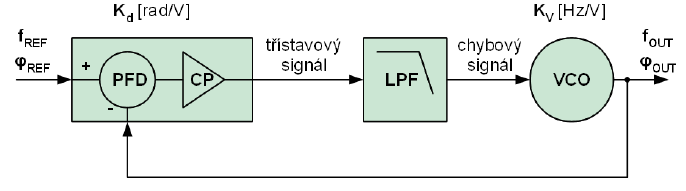
\includegraphics[scale=0.55]{Obrazky/VFT/schema_fazovho_zavesu.png}}
		\captionsetup{justification=centering}
		\caption{Blokové schéma fázového závesu}
		\label{}
	\end{figure}
	
	{\raggedright \textbf{Fázovo frekvenčný detektor}}\\
	-- sú založené na dvojici klopných obvodov typu D \\
	-- sú riadené nábežnou hranou vstupných signálov \\
	-- výstupy klopných obvodov sú pripojené na nábojovú pumpu, ktorá umožňuje generovať trojstavový signál s úrovňami -1, 0, 1\\
	-- vstupy a výstupy: REF, OUT, trojstavový sginál (-1,0,1)
	
	\begin{figure}[H]
		%\vspace{-2mm}
		\makebox[\textwidth]{%
			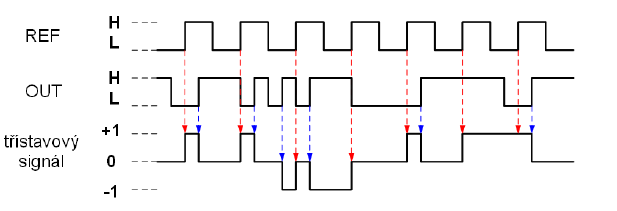
\includegraphics[scale=0.5]{Obrazky/VFT/fazovo_frek_detektor.png}}
		\captionsetup{justification=centering}
		\caption{Signál na výstupe nábojovej pumpy v závislosti na vstupných signáloch PFD}
		\label{}
		%\vspace{-2mm}
	\end{figure}
	-- napätie na ladiacom vstupe VCO sa zvyšuje, čo odpovedá poklesu kapacity ladiacého varikapu vnútri VCO a tým zvýšenie výstupného kmitočtu VCO \\
	%\vspace*{2mm}
	{\raggedright \textbf{Filter slučky}}\\
	-- je charakterizovaný prenosovou funkciou dolnej priepuste a je určený pre potlačenie vysokofrekvenčných zložiek výstupného signálu PFD\\
	-- parametre výrazne ovplyvňujú správanie celého systému a majú vplyv najmä na dynamické vlastnosti PLL \\
	-- návrh filtra ovplyvňuje: odozvu systému na skokové zmeny referenčnej frekvencie, stabilita alebo fázový šum výstupného signálu \\
	-- používajú sa pasívne aj aktívne RC filtre rôznych radov\\
	-- filter slučky zavádza do spätnoväzobného systému určitú zotrvačnosť, ktorá sa prejavuje pri skokovej zmene referenčnej frekvencie \\
	
		
	\begin{figure}[H]
		%\vspace{-2mm}
		\makebox[\textwidth]{%
			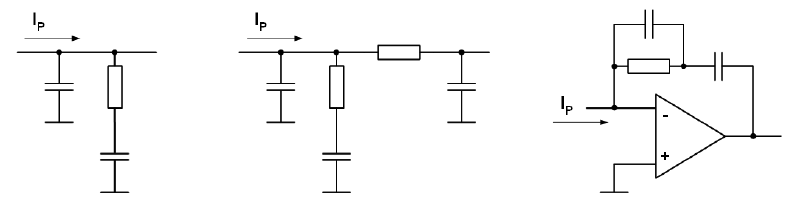
\includegraphics[scale=0.55]{Obrazky/VFT/filter_smycky.png}}
		\captionsetup{justification=centering}
		\caption{Príklady zapojenia filtra pre PLL s nábojovou pumpou}
		\label{}
	\end{figure}

	V závislosti na šírke pásma filtru slučky vykazuje fázový záves tieto vlastnosti:\\
	\textbf{Malá šírka pásma}:\\
		-- systém je necitlivý vôči rýchlym zmenám frekvencie\\
		-- malá schopnosť synchronizácie pri zmene kmitočtu\\
	
	\textbf{Veľká šírka pásma}: \\
	-- systém sleduje rýchle zmeny referenčnej frekvencie \\
	-- rýchla synchronizácia na nový kmitočet \\
	%\vspace{2mm}
	{\raggedright \textbf{Výstupný signál PLL syntetizátora pri zmene frekvencie:}}
	
	\begin{figure}[H]
		%\vspace{-2mm}
		\makebox[\textwidth]{%
			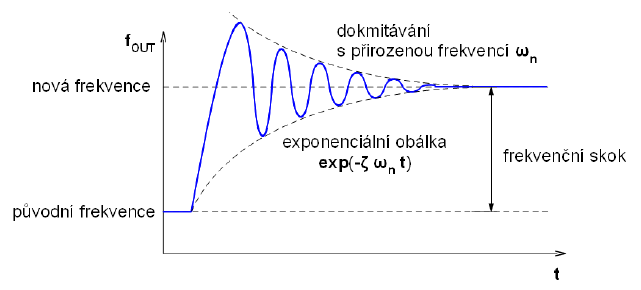
\includegraphics[scale=0.4]{Obrazky/VFT/odozva_zmeny_frek.png}}
		\captionsetup{justification=centering}
		\caption{Príklady zapojenia filtra pre PLL s nábojovou pumpou}
		\label{}
	\end{figure}
	
	- pri skokovej zmene sa výstupný kmitočet systému ustaluje na novú hodnotu dokmitávaním s prirodzenou frekvenciou
	  $\omega_n$ a časovou konštantou, ktorá je daná činiteľom tlmenia $\xi$\\
	- dĺžka dokmitávania je daná filtrom slučky a veľkosťou skokovej zmeny frekvencie\\
	%\vspace{-2mm}
	\subsubsection{Syntetizátor s celočíselným deliacim pomerom N (Integer-N):}
	\textbf{a.) Syntetizátor s pevným preddeličom}\\
	- na jeden vstup PFD je privedený kmitočet $f_1$, ktorý vznikne delením referenčného signálu deliacím pomerom R \\
	- na druhý vstup je privedený kmitočet $f_2$, ktorý vznikne delenm výstupného signálu VCO pevným preddeličom P a nastaviteľným deličom N
	
	\begin{figure}[H]
		%\vspace{-2mm}
		\makebox[\textwidth]{%
			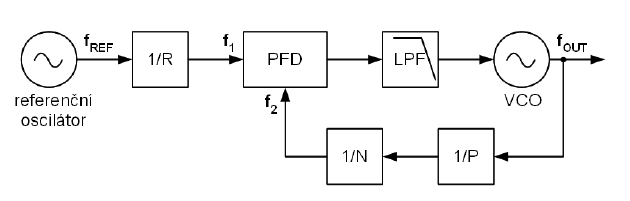
\includegraphics[scale=0.5]{Obrazky/VFT/syntetizator_pevny_preddelic.png}}
		\captionsetup{justification=centering}
		\caption{PLL syntetizátora s pevným preddeličom P a nastaviteľným deličom N}
		\label{}
	\end{figure}
	
	Výstupný kmitočet syntetizátora:
	\begin{equation}
		f_{out} = \frac{f_{ref}}{R} \cdot P\cdot N
	\end{equation}
	P - deliací pomer preddeliča
	N - nastaviteľný delič
	R - deliací pomer ($f_{ref}$)
	
	Kmitočtový krok $\Delta f$:
	\begin{equation}
		\Delta f = f_{OUT}^{N+1} - f_{OUT}^{N} = \frac{f_{ref}}{R} \cdot P
	\end{equation}

	\textbf{b.) Syntetizátor s riadeným preddeličom\\}
	- využíva preddelič, ktorý je schopný prepínať deliací pomer medzi hodnotami $P$ a $(P+1)$\\
	- v spätnej väzbe sú zapojené dva čítače o dĺžke $A$ a $B$ bitov\\
	- preddelič a obe čítače tvoria riadiacu logiku a jeho celkový deliaci pomer je označený N
	\begin{figure}[H]
		%\vspace{-2mm}
		\makebox[\textwidth]{%
			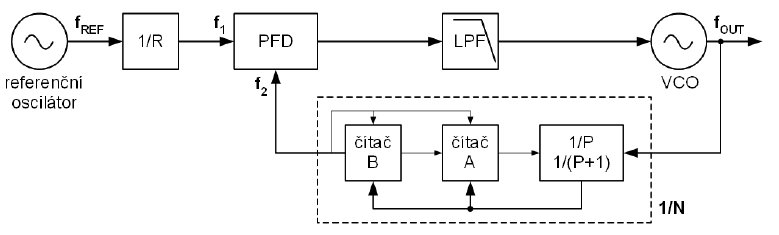
\includegraphics[scale=0.5]{Obrazky/VFT/syntetizator_riadeny_preddelic.png}}
		\captionsetup{justification=centering}
		\caption{PLL syntetizátor s riadeným preddeličom}
		\label{}
	\end{figure}
	
	\textbf{Funkcie bloku N:}\\
	  1. Čítače A a B sú vynulované a preddelič je nastavený na deliaci pomer (P + 1)\\
	  2. Oba čítače čítajú impulzy signálu deleného pomerom (P+1) dokedy čítač A nedosiahne maximálnej hodnoty $A_{max}$ \\
	  3. Deliací pomer preddeliča je prepnutý na $P$ a čítač $B$ pokračuje v čítaní signálu deleného P dokedy nedosiahne maximálne hodnoty $B_{max}$. \\	
	  4. proces sa opakuje\\
	  	%\vspace{2mm}
\textbf{Výstupný kmitočet:}
	\begin{equation}
		f_{out} = \frac{f_{ref}}{R} \cdot (A+P\cdot B)
	\end{equation}

	\textbf{Kmitočtový krok }$\Delta f$:
	\begin{equation}
		\Delta f = \frac{f_{ref}}{R}
	\end{equation}
	
	
	\textbf{Výhoda riadeného preddeliča:}\\
	- výhodou tohto systému je, že preddelič nemá vplyv na veľkosť kmitočtového kroku $\delta f$ a nezhoršuje tak frekvenčne rozlíšenie\\
	
	\medskip
	\subsubsection{Syntetizátor s neceločíselným deliacím pomerom N}
	- je schopný pracovať s veľmi jemným kmitočtovým krokom, ktorý je nezávislý na veľkosti deliaceho pomeru R\\
	- využíva nastaviteľné deličky N, ktoré je schopná podľa určitej priemerovacej funkcie prepínať medzi deliacím pomerom N a (N+1) tak, že výsledkom je neceločíselný deliaci pomer $N_F$\\
	\medskip
	\textbf{Výhody}:\\ -- väčšia rýchlosť ustálenia výstupného signálu pri preladení a nižší fázový šum výstupného signálu \\
	\medskip
	\textbf{Nevýhody}: 
	\begin{itemize}[label=--]
	%\vspace{-4mm}
	\item nikdy nedôjde k ustáleniu kmitočtu v spätnej väzbe a detektor sa snaží chybu korigovať \\		  
	\item vyššia četnosť, vyššia úroveň diskrétnych rušivých signálov vo výstupnom spektre syntetizátora
	\end{itemize}
  \newpage
	\textbf{Fázový šum a spektrum PLL syntetizátora:}
	
		\begin{figure}[H]
		%\vspace{-2mm}
		\makebox[\textwidth]{%
			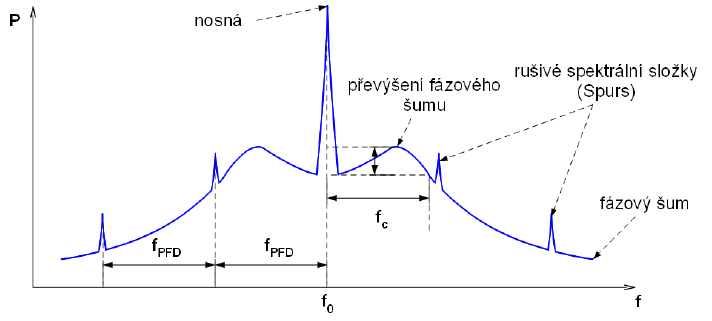
\includegraphics[scale=0.4]{Obrazky/VFT/spektrum_pll_syntetizatora.png}}
		\captionsetup{justification=centering}
		\caption{Spektrum výstupného signálu PLL syntetizátora s celočíselným deliacim pomerom N}
		\label{}
	\end{figure}
	- okrem hlavnej spektrálnej čiary sú v blízkosti prítomne rušíve zložky, ktoré majú pôvod v preddelenom referenčnom signále, ktorý je privádzaný na vstup fázovo frekvenčného detektora\\
	- vo spektre sa periodicky opakuje s odstupom $f_{PFD} = f_1$ a ich amplitúda so vzdialenosťou od nosnej klesá.

	\subsubsection{Princíp DDS syntetizátora}
	- časový priebeh je v číslicovej forme a s potrebným rozlíšením uložený v pamäti ROM (lookup tabuľke)\\
	- Z tej sú vypočítane jednotlivé hodnoty (vzorky) časového priebehu signálu a prostredníctvom D/A prevodníka sú prevedené na výstupný analógový signál
	
	\begin{figure}[H]
		%\vspace{-2mm}
		\makebox[\textwidth]{%
			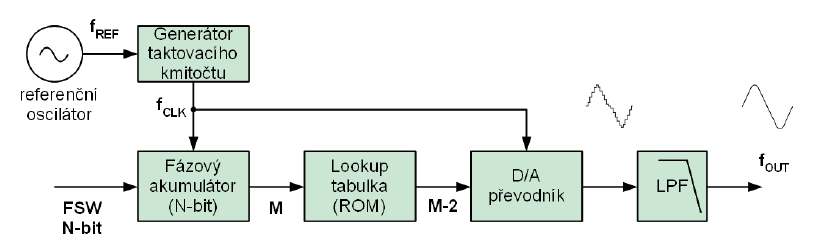
\includegraphics[scale=0.4]{Obrazky/VFT/DSS_syntetizator.png}}
		\captionsetup{justification=centering}
		\caption{Blokové schéma DDS syntetizátora}
		\label{}
	\end{figure}
	
	Výstupný kmitočet:
	\begin{equation}
		f_{OUT} = \frac{FSW}{2^N} \cdot f_{CLK}
	\end{equation}
	
	FSW - N bitové riadiacé slovo, N - počet bitov slova, $f_{CLK}$ - riadiací hodinový signál\\
	\medskip
	\textbf{Fázový akumulátor}\\
	-- jedna sa o čítač, ktorého dĺžka je N bitov a ktorého obsah je aktualizovaný s každou periódou taktovacieho signálu $f_{CLK}$\\ 
	-- úlohou fázového akumulátora je generovanie adresy vzorku pre lookup tabuľku aktuálnej fáze funkcie sinus\\
	\medskip
	\textbf{Výstupný filter}\\
	-- antialiasingový filter, ktorý je zaradený na výstup D/A prevodníka \\
	-- má za úlohu potlačiť zrkadlové signály, ktoré podľa vzorkovacieho teorému vznikajú symetricky okolo násobku vzorkovacej frekvencie D/A prevodníka \\
	\newpage
	\textbf{Vlastnosti spektra DDS synstetizátora} \\
	-- spektrum DDS syntetizátora obsahuje nežiadúce zložky \\
	-- najväčšiu amplitúdu majú takzvané zrkadlové signály, ktoré sa podľa vzorkovacieho teorému vo spektre \\
	  opakujú okolo násobku vzorkovacej frekvencie prevodníka \\
	-- zrkadlové signály sú na kmitočtoch $f_{CLK} - f_{OUT}$ a $f_{CLK} + f_{OUT}$
	
	\begin{figure}[H]
		%\vspace{-2mm}
		\makebox[\textwidth]{%
			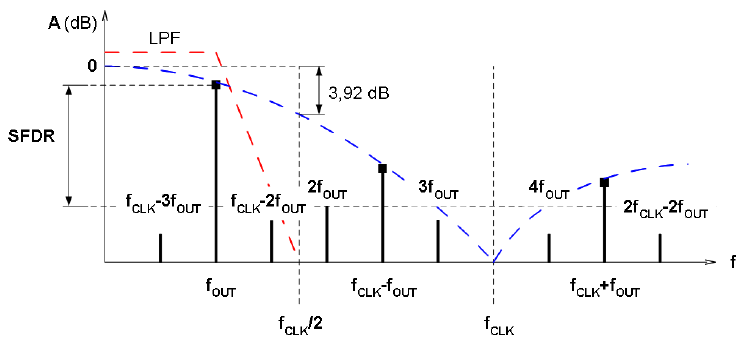
\includegraphics[scale=0.4]{Obrazky/VFT/spektrum_dds.png}}
		\captionsetup{justification=centering}
		\caption{Výstupné spektrum DDS syntetizátora}
		\label{}
	\end{figure}
	
%\end{document}



 